\chapter{Earth Faults in \SI{110}{\kilo\volt} and \SI{10}{\kilo\volt} Power Grids}
\label{chap:earth-faults}
\index{earth fault}
\index{Petersen coil}
\index{resonant grounding}
\index{neutral displacement voltage}

\section{General}
\label{sec:earth-fault-general}

A Petersen coil is an intelligent protection and stabilization element in medium-voltage networks and, in some cases, also in high-voltage networks. It ensures that single-phase earth faults can be controlled safely and without immediate shutdown. This makes it an indispensable component of modern power supply systems.
The Petersen coil is an inductive coil that is connected to the neutral point of the transformer. In a three-phase AC network, capacitive currents flow between conductors and earth. If a ground fault occurs, a capacitive fault current flows through the fault location – this can be dangerously high.
In the event of a fault, the Petersen coil generates an inductive current that is opposes the capacitive fault current and, in the ideal case, compensates for it at the fault location.

\section{Circuit design}

This chapter investigates earth faults in small cable networks with resonant neutral grounding. The first example is the simulation file \texttt{Petersen\_without\_Fault\_TRAN.asc}. The principal \SI{110}{\kilo\volt} example is designed for
a nominal earth-fault compensation current of \SI{300}{\ampere}. In normal
operation, network asymmetry produces only a small neutral displacement
voltage and therefore a small Petersen-coil current. During a solid earth
fault, approximately the full phase-to-earth voltage appears between the
transformer neutral and earth, and the coil supplies approximately its rated
current.

Unless stated otherwise, the transformer is unloaded. The earth fault is
applied at \SI{205}{\milli\second}. The voltage-source parameter
\texttt{texp} is used to establish steady state rapidly before the fault. The
model contains a Yd5 transformer whose parameters are defined in the LTspice file \texttt{Transformer\_110k\_10k.asc}

\section{Compensated \SI{110}{\kilo\volt} Network Without a Fault}
\label{sec:Compensated Network Without a Fault}

\subsection{Adjustment of the Petersen Coil}
\label{sec:Adjustment of the Petersen Coil}

The network has a phase-to-earth capacitance of \SI{5012}{\nano\farad} per phase. At \SI{50}{\hertz}, its capacitive reactance is ..

\begin{calculation}{Petersen-coil rating from the network capacitance}{calculation51}
\begin{align}
X_C&=\frac{1}{\omega C}
 =\frac{1}{2\pi\cdot\SI{50}{\hertz}\cdot\SI{5012}{\nano\farad}}
 \approx\SI{635.1}{\ohm},\\
I_C&=\frac{U_{\mathrm{LL}}/\sqrt{3}}{X_C}
 =\frac{\SI{110}{\kilo\volt}/\sqrt{3}}{\SI{635.1}{\ohm}}
 \approx\SI{100}{\ampere}\ \text{RMS}.
\end{align}

For a single-phase earth fault, the total capacitive earth-fault current is
approximately three times the phase charging current. Resonant compensation
therefore requires

\begin{align}
I_{\mathrm P}&\approx3I_C=\SI{300}{\ampere},\\
X_{L,\mathrm P}&=\frac{X_C}{3}
 \approx\boxed{\SI{211.7}{\ohm}}.
\end{align}
\end{calculation}

The Petersen-coil model accepts the nominal line-to-line voltage and
compensation current directly. We set these to \SI{110}{\kilo\volt} and
\SI{300}{\ampere}.

\subsection{Neutral Displacement Voltage in the Transient Analysis}
\label{sec:Neutral Displacement Voltage in the Transient Analysis}

Even without a fault, unequal phase-to-earth capacitances produce a neutral
displacement voltage across the Petersen coil. In this example, its peak value is
approximately \SI{1.2}{\kilo\volt} peak, much smaller than the rated phase voltage.
The greater the difference between the phase capacitances, represented in the
model by \texttt{CE+CE1} and \texttt{CE}, the higher this voltage becomes.

The displacement voltage rises slowly and shows a beat frequency of
approximately \SI{1.2}{\hertz}. This indicates that the resonant frequency is
not exactly \SI{50}{\hertz}. In the LTspice waveform viewer, the beat frequency
can be read by drawing a zoom window between two adjacent maxima and observing
the frequency in the status line. (See figure \ref{fig:Figure1})
 

\subsection{Corrected Petersen-Coil Setting}
\label{sec:Corrected Petersen-Coil Setting}

The capacitance-only calculation in calculation \ref{calc:calculation51} is correct for
an ideal transformer, but the complete resonant circuit is not optimally compensated
with a \SI{300}{\ampere} coil. The transformer short-circuit reactance on the primary side,
$X_{\mathrm{1s}}=\SI{30.25}{\ohm}$ (see \texttt{Transformer\_110k\_10k.asc}) , reduces the
resonant frequency to \SI{48.8}{\hertz}. The coil nominal current must
therefore be increased to approximately \SI{315}{\ampere} to get again \SI{50}{\hertz}. This can be verified by simulating with \texttt{Petersen\_without\_Fault\_AC.asc}. (See figure \ref{fig:Figure2})

Now we set the initially choosen value of
1E20 for the magnetic reluctance of the transformer tank to a reasonable value of 1e6. After running the simulation, we find that the resonant frequency is again below \SI{50}{\hertz}. 

We now choose \SI{328}{\ampere} for the Petersen coil. We restart the simulation. Now we see that the resonant point is again at approximately \SI{50}{\hertz}. We have seen now that the compensation current calculated from the total cable capacitance alone differs from the required Petersen-coil setting because of the transformer’s internal impedance. We have to add about 10\% for the Petersen current value to compensate for the voltage drop at the starpoint.

\begin{remark}{Phase information in AC analysis}{rem:automatic-Petersen}
	In practice, the automatic Petersen-coil controller normally maintains slight overcompensation or undercompensation to avoid resonance. Additionally the controller is disabled when an earth fault occurs to prevent further drift.
\end{remark}

\subsection{Reason about the reduction of the starpoint voltage}
 
Explanation of the Reduced Neutral-Point Voltage when adding the magnetic reluctance of the transformer tank lies in the additional secondary leakage flux and the corresponding voltage drop across the leakage reactance. This further decreases the effective neutral‑point voltage.
You can clearly see this in the file \texttt{Petersen\_with\_fault\_hierarchical\_model\_AC.asc}. After simulation click on the transformer symbol then open schematic. Then click on the symbol for the primary winding Phase A and open schematic again. Then measure the current through RPhis. This gives approximately 9 mA (This current models the flux value in Wb). Perform the same measurement for the secondary winding above the primary winding. The current there is 7 mA increasing now the sum of all leakage fluxes. The Resonant frequency is approximately 47.9Hz. (See figure \ref{fig:Figure4})


\subsection{Resonance Frequency at about 50Hz}
\label{sec:Resonant Frequency at about 50Hz}
This is the resonance of all three phase capacitances with the Petersen-coil
inductance and the effective transformer leakage inductance in the
zero-sequence path. The coil reactance and inductance are

\begin{align}
	X_{\mathrm P}&=\frac{U_{\mathrm{LL}}}{\sqrt{3}I_{\mathrm P}}
	=\frac{\SI{110}{\kilo\volt}}{\sqrt{3}\cdot\SI{300}{\ampere}}
	\approx\SI{211.7}{\ohm},\\
	L_{\mathrm P}&=\frac{X_{\mathrm P}}{2\pi\cdot\SI{50}{\hertz}}
	\approx\SI{0.674}{\henry}.
\end{align}

The transformer leakage reactance gives

\begin{equation}
	L1s=\frac{\SI{30.25}{\ohm}}
	{2\pi\cdot\SI{50}{\hertz}}\approx\SI{0.096}{\henry}.
\end{equation}

Since the three phase capacitances act in parallel and the three transformer
phase inductances contribute as $L1s_{}/3$ 


\begin{calculation}{Resonanz at 50Hz without leakage inductance}{Calculation52}
	\begin{align}
		C_0&=3\cdot\SI{5012}{\nano\farad},\\
		L_0&=L_{\mathrm P}+\frac{L1s}{3}
		=\SI{0.674}{\henry},\\
		f_{\mathrm r,0}&=\frac{1}{2\pi\sqrt{L_0C_0}}
		\approx\boxed{\SI{50}{\hertz}}.
	\end{align}
\end{calculation}

\begin{calculation}{Resonanz at 48.8Hz with primary leakage inductance}{Calculation53}
	\begin{align}
		C_0&=3\cdot\SI{5012}{\nano\farad},\\
		L_0&=L_{\mathrm P}+\frac{L1s}{3}
		=\SI{0.674}{\henry}+\frac{\SI{0.096}{\henry}}{3},\\
		f_{\mathrm r,0}&=\frac{1}{2\pi\sqrt{L_0C_0}}
		\approx\boxed{\SI{48.8}{\hertz}}.
	\end{align}
\end{calculation}

\begin{calculation}{Resonanz at 47.9Hz also with secondary leakage inductance}{Calculation54}
	\begin{align}
		C_0&=3\cdot\SI{5012}{\nano\farad},\\
		L_0&=L_{\mathrm P}+\frac{L1s}{3}+\frac{L1s*7}{9}
		=\SI{0.674}{\henry}+\frac{\SI{0.096}{\henry}}{3}+\frac{\SI{0.096}{\henry}*7}{9},\\
		f_{\mathrm r,0}&=\frac{1}{2\pi\sqrt{L_0C_0}}
		\approx\boxed{\SI{47.95}{\hertz}}.
	\end{align}
\end{calculation}

7/9 means the relation of the leakage fluxes measured above (9 Wb and 7 Wb).  
The resonant peaks for 48.8 Hz and 47.95 Hz can also be observed in the file\\
\texttt{Petersen\_without\_fault\_AC.asc}. 
by setting rkessel (this is the parameter for tank reluctance) to 1e6 or 1e20.
For the calculation of the resonant frequencies see also the file \texttt{Petersen.asc}



\section{Low-Resistance Earth Fault in the \SI{110}{\kilo\volt} Network}
\label{sec:110kv-low-resistance-earth-fault}

\subsection{Network Compensated with \SI{328}{\ampere} }
\label{sec:300a-earth-fault}

The transient simulation is contained in
\texttt{Petersen\_with\_fault\_TRAN.asc} (see figure \ref{fig:Figure5a}). At fault inception, the phase-R voltage
rapidly collapses to zero. The voltages of the two healthy phases rise toward
the line-to-line voltage. This transition is accompanied by high-frequency
overvoltages and currents. An FFT shows a mixture of dominant components near
\SI{260}{\hertz} and \SI{1.2}{\kilo\hertz}. (see figure \ref{fig:Figure13}) .

At this higher frequency, the capacitive reactance decreases and the
inductive reactance of the line impedance increases. The capacitive current
through the inductive impedance therefore produces an additional voltage rise.
The currents flowing toward the transformer are predominantly inductive and
approximately in phase with one another. Their inductive character can be
recognized because the current maximum lags the corresponding voltage maximum.
You can also see that the voltages of the healthy phases have a phase difference going from
120 degrees to 60 degrees (see figure \ref{fig:FigureX})

The current at the fault location initially reaches approximately
\SI{4.2}{\kilo\ampere} peak (see figure \ref{fig:Figure5}). It decays rapidly and approaches approximately a steady-state peak value of approximately \SI{4}{\ampere} peak. Its minimum also depends on the ohmic resistance of the Petersen coil, set by \texttt{r\_x} parameter.
The prefault capacitive reactive power is approximately \SI{-6.3}{\mega\varunit} per phase, or about
\SI{-19}{\mega\varunit} in total. Immediately after the phase A fault, the
high-frequency recharging process briefly drives the phase B and phase C
values to approximately \SI{-40}{\mega\varunit}. However, immediately after the fault. The capacitive and inductive reactive-power components are superimposed. The reason for the doubling of the capacitive reactive power is that the two
capacitances of the healthy phases are suddenly subjected to a voltage √3 times the normal phase-to-earth voltage. At the end of the transient processes, the additional capacitive reactive power is again compensated by the Petersen reactor. In addition, the inductive reactive power decays to zero. In the end, the reactive power is exactly the same as it was at the beginning (see figure \ref{fig:Figure5} and \ref{fig:Figure6}). In \texttt{Petersen\_with\_Fault\_AC.asc}, the minimum fault
current is approximately \SI{3}{\ampere} RMS near \SI{50}{\hertz} (see figure \ref{fig:Figure6}). Set the vertical axis to linear scaling to read this minimum accurately.
You can also see that the voltage magnitude of phase A is zero, and that Phase B and Phase C are at 111 kV, which is the phase‑to‑phase voltage.The phase angle of phase B is −150°, and that of phase C is +150°. The difference is −150 − 150 = −300 = +60 degrees, just as we observed earlier. (see figure \ref{fig:FigureX})


 


\begin{remark}{Phase information in AC analysis}{rem:earth-fault-ac-phase}
The relative phase angles of voltages and currents are most accurately
examined in the AC-analysis files, where the fundamental-frequency phasors are
not obscured by the switching transient.
\end{remark}

\subsection{Reactive Power detailed}
\label{sec:earth-fault-reactive-power}

The capacitive reactive power of the network is approximately

\begin{equation}
	Q_C=\sqrt{3}\,U_{\mathrm{LL}}I_C
	=\sqrt{3}\cdot\SI{110}{\kilo\volt}\cdot\SI{100}{\ampere}
	\approx\SI{19}{\mega\varunit}.
	\label{eq:network-capacitive-reactive-power}
\end{equation}

It can be measured with the \texttt{qmeter\_uvw} element. Each phase contributes
approximately \SI{-6.3}{\mega\varunit}, with small differences caused by the
unequal capacitances and the resulting unequal phase voltages (This explains the neutral displacement voltage). The waveform
viewer shows approximately \SI{110}{\kilo\volt},
\SI{111.7}{\kilo\volt}, and \SI{110.7}{\kilo\volt} after the model's display
scaling by $\sqrt{3}/\sqrt{2}$. Their mean is slightly above
\SI{110}{\kilo\volt} because the capacitive current produces a voltage rise
across the inductive line impedance.

\begin{remark}{Waveform-viewer units and scaling}{rem:qmeter-scaling}
	Multiplying a power trace by \texttt{1W/1V} can be used to change the displayed
	unit prefix in the waveform viewer. If \texttt{sfactor=3} is selected in
	\texttt{qmeter\_uvw}, the measured values are multiplied internally by three,
	which may simplify comparison with the total three-phase power.
\end{remark}


\subsection{Reactive-Power Increase at Fault Inception}
\label{sec:earth-fault-reactive-power-doubling}

During the earth fault, the two healthy phase-to-earth capacitances are charged
to approximately the line-to-line voltage, while the capacitance of the
faulted phase is discharged. Since capacitive reactive power is proportional
to voltage squared, the total capacitive reactive power of the healthy phases
is ideally twice (because of the voltage transients even higher) the prefault three-phase value. The source current therefore
also rises correspondingly.

After the transient, one part of this increased capacitive earth-fault current
is compensated by the Petersen coil. The ordinary positive-sequence charging
current remains supplied by the source.


\subsection{Additional Transformer Loading Due to Petersen-Coil Current}
\label{sec:petersen-transformer-loading}

The Petersen-coil current flows through the transformer windings and therefore
adds to the transformer loading. In the example, its equivalent contribution
is approximately \SI{100}{\ampere} per phase, while the rated primary current
is approximately \SI{200}{\ampere}. Because this current is predominantly
inductive, it must be added vectorially to the load current. For the assumed
load, whose reactive component is about one fifth of its active component,
approximately \SI{90}{\percent} of the original load capability remains.
NOTE: The additional load due to the Petersen is only present when a earth-fault
occur. In addition, we must take into account the high secondary-side circulating current resulting from the inclusion of the transformer tank in the simulation which also puts a  certain load on the transformer.
This is seen best in the file \texttt{Petersen\_without\_fault\_hierarchical\_model\_TRAN/AC.asc}.
Right-click the transformer symbol and select \texttt{Open Schematic}. After running the simulation, measure the current in the secondary winding of Phase A. 

\subsection{Loaded and Unloaded Transformer}
\label{sec:loaded-unloaded-transformer-earth-fault}

Changing the load parameter from \texttt{20e-6} to \texttt{40e6} reduces both
the phase voltages and the transformer neutral voltage. Since the voltage
across the cable capacitances decreases at the same time, the compensation
tuning remains almost unchanged. The comparison is implemented in
\texttt{Petersen\_with\_fault\_with\_load\_vs\_without\_load\_AC.asc}.
(see figure \ref{fig:Figure7a} and \ref{fig:Figure7})
NOTE: The Petersen current in the unloaded case is higher (304A) because of higher voltage level of 111.4kV compared to the loaded case where the voltage level is 110kV and the current is (300A). 

\section{High-Resistance Earth Fault}
\label{sec:110kv-high-resistance-earth-fault}

The AC-analysis file \texttt{Petersen\_with\_fault\_highohmic\_AC.asc}
compares the earth-fault resistances \SI{50}{\ohm}, \SI{100}{\ohm},
\SI{500}{\ohm}, and \SI{1000}{\ohm}. At the resonance point, all current
curves approach approximately \SI{3}{\ampere}, representing the residual
ohmic component of the compensated earth-fault current.
(see figure \ref{fig:Figure8a} and \ref{fig:Figure8})

\section{Comparison of coupled and uncoupeled line impedance}
\label{sec:coupled-uncoupled}
Open \texttt{Petersen\_fault\_coupled\_uncoupled.asc} and run the simulation.
After simulation we see that the peak fault current is lower in the coupled-line case than in the uncoupled-line case. The difference is about \SI{1}{\kilo\ampere}. The steady state current at the end of the simulation is the same for the two cases. 
This shows that simulating a asymmetric fault the coupling of the lines has to be
considered. For the calculation of the coupled impedance values see also the wxmaxima file \texttt{Petersen.asc}\\
(see figure \ref{fig:Figure9a} and \ref{fig:Figure9})

\begin{important}{Asymmetric faults}{}
	Coupling must be included when simulating asymmetrical faults in coupled-line systems.
\end{important}


\section{Compensated \SI{10}{\kilo\volt} Network with a Grounding Transformer}
\label{sec:grounding-transformer}
A Yd transformer does not provide an accessible neutral on its delta-connected
side. An external neutral-forming transformer, represented by
\texttt{Trafo\_gnd} symbol, creates a neutral point in the medium-voltage network without presence of a transformer with starpoint so that a Petersen coil can be connected. The corresponding simulation files are

\begin{itemize}
	\item \texttt{Petersen\_Trafo\_gnd\_TRAN.asc},
	\item \texttt{Petersen\_Trafo\_gnd\_AC\_fault.asc},
	\item \texttt{Petersen\_Trafo\_gnd\_AC\_no\_fault.asc}.
\end{itemize}

We now see a \texttt{\SI{10}{\kilo\volt}} compensated network with external grounding transformer. You see a Petersen in a medium voltage network. Due to the star point builder, a YD transformer can establish a star point at the secondary side for connecting a Petersen coil. 

\section{Petersen-coil and Yy-Transformers with three legs} 

Now consider a Petersen coil connected to a Yy transformer with a three-leg core. Since the YY transformer has no low-reluctance return path for zero-sequence flux in the core of the transformer, the flux must return through the tank and oil. This is not the goal. Therefore, the star point of a wye/wye transformer should only be loaded to no more than 10\% of the transformer’s rated current. See \texttt{ThreeLegCore-Yy-Transformer.asc}

\section{Solid Neutral Earthing and a Yy-Transformer with a Five-Leg Core}
Open the File \texttt{FiveLegCore\_without\_third\_winding.asc}. If the Yy-transformer has a five leg core, the star point cannot deliver any current if the second star point is isolated. This is because the outer legs provide a low-reluctance return path for in-phase fluxes. If the second star point is also connected, current can flow from one into the other star points, but current should not be exchanged between the two star points. In short, the two star points of a five leg Yy-transformer should be isolated. Now open file \texttt{FiveLegCore\_with\_third\_winding.asc}. Now consider neutral-point loading in a Yy transformer with a five-leg core and a compensating tertiary winding. The transformer can deliver full current at the star points. There is also no current transfer from one to the other star point.

\section{Characteristic Resonance Frequencies}
\label{sec:earth-fault-resonance-frequencies}

Several natural frequencies occur after fault inception. The highest is
associated with the discharging capacitance of the faulted phase. A lower
frequency appears in the healthy-phase voltages and capacitance currents.



\subsection{Resonance at \SI{1.2}{\kilo\hertz}}

This resonant path contains the cable series inductance and the faulted phase
capacitance. It is driven mainly through capacitor C12 and the fault position.
With $L=\SI{3.5}{\milli\henry}$ and
$C=\SI{5022}{\nano\farad}$ follows ..

\begin{equation}
	f_{\mathrm r}=\frac{1}{2\pi\sqrt{LC}}
	\approx\boxed{\SI{1.2}{\kilo\hertz}}.
\end{equation}


\subsection{Resonance at \SI{260}{\hertz}}

This is the frequency of the current through the netimpedance
and the capacities C10 and C11.
With $L=\SI{25}{\milli\henry}$ and $C=\SI{5012}{\nano\farad}$*3


\begin{equation}
	f_{\mathrm r}=\frac{1}{2\pi\sqrt{LC}}
	\approx\boxed{\SI{260}{\hertz}}.\\
\end{equation}

For the frequencies see figure \ref{fig:Figure13}

\begin{figure}[H]
	\centering
	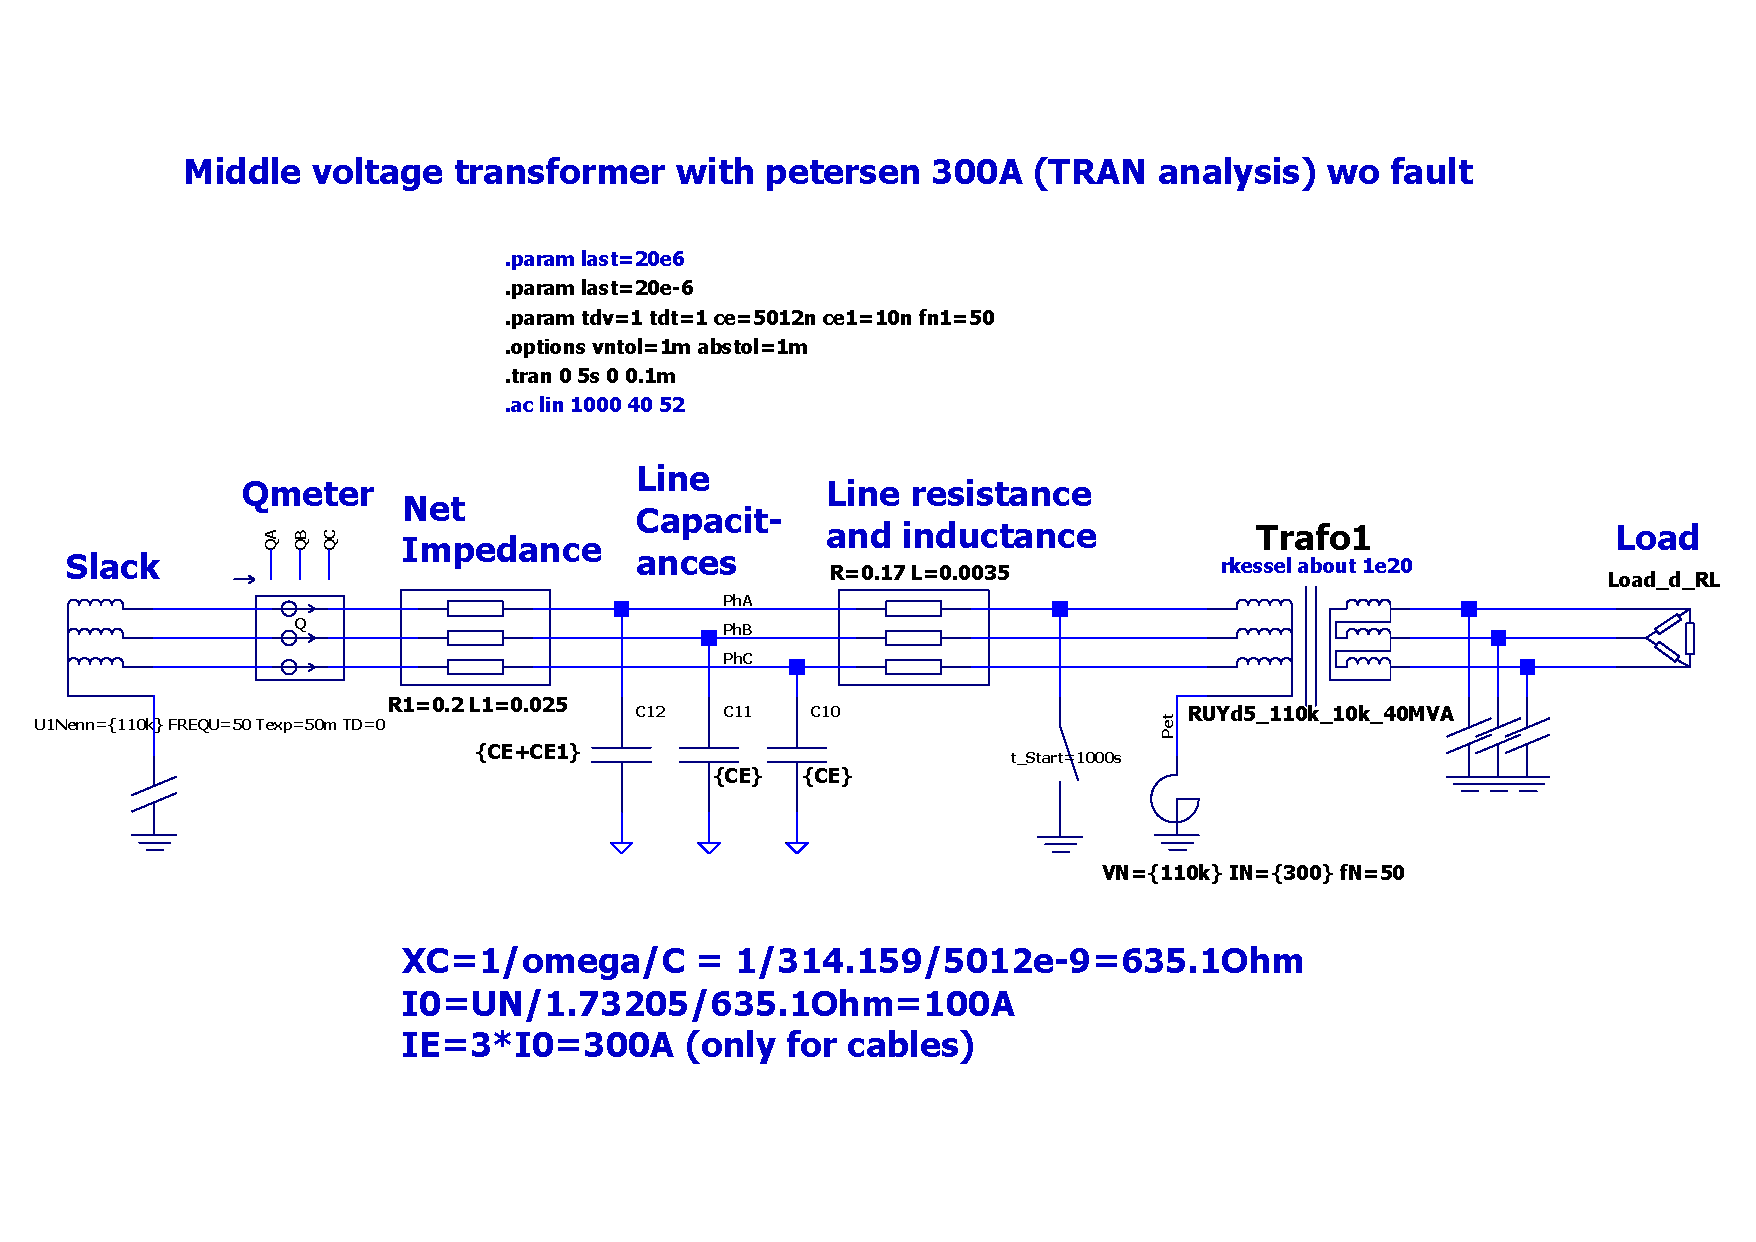
\includegraphics[width=0.90\textwidth]{figures/05_Petersen_earth_faults/Petersen_without_fault_TRAN_schematic}
	\caption{Petersen without fault - schematic}
	\label{fig:Figure1a}
\end{figure}

\begin{figure}[H]
	\centering
	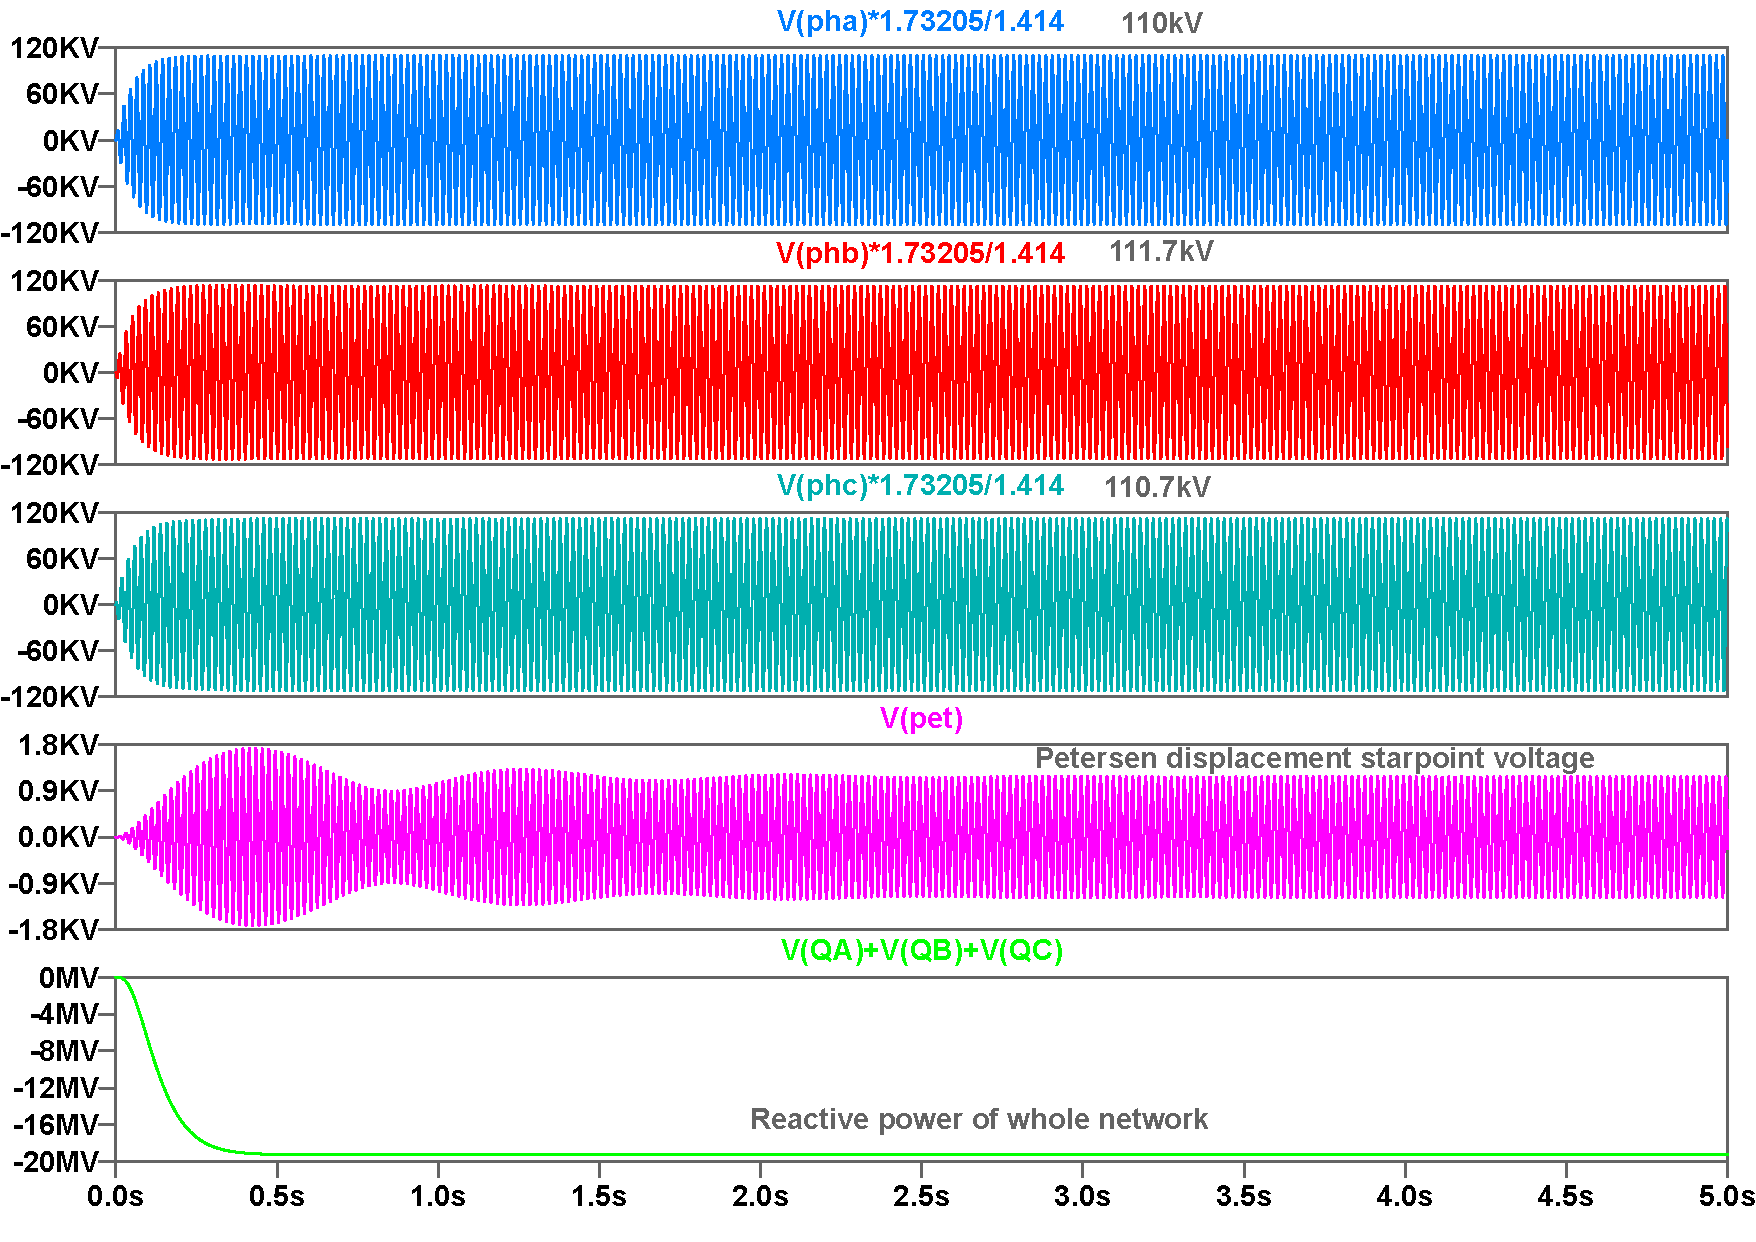
\includegraphics[width=0.90\textwidth]{figures/05_Petersen_earth_faults/Petersen_without_fault_TRAN_waveform.pdf}
	\caption{Petersen without fault TRAN - waveform}
	\label{fig:Figure1}
\end{figure}



\begin{figure}[H]
	\centering
	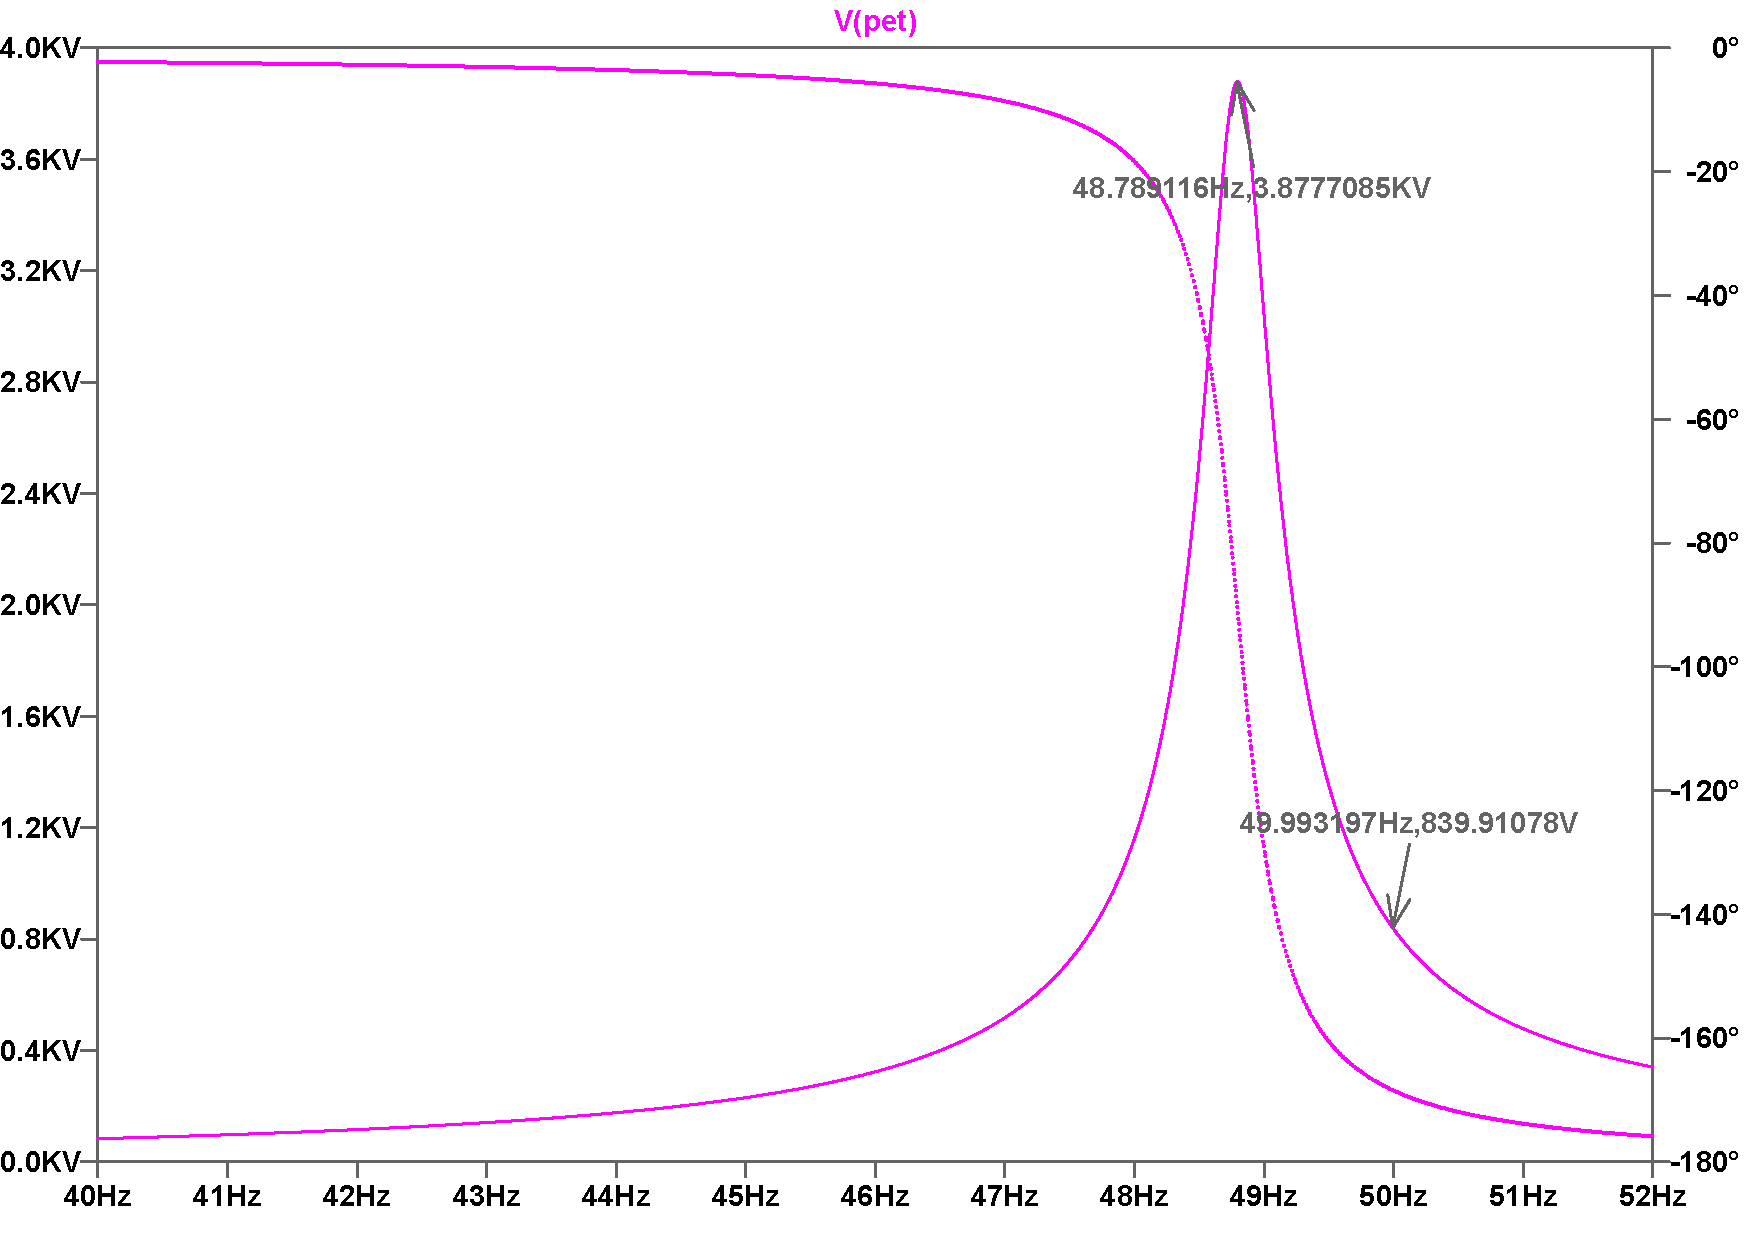
\includegraphics[width=0.90\textwidth]{figures/05_Petersen_earth_faults/Petersen_without_fault_AC_waveform.pdf}
	\caption{Petersen without fault AC starpoint (Petersen) voltage - waveform}
	\label{fig:Figure2}
\end{figure}

%\begin{figure}[H]
%	\centering
%	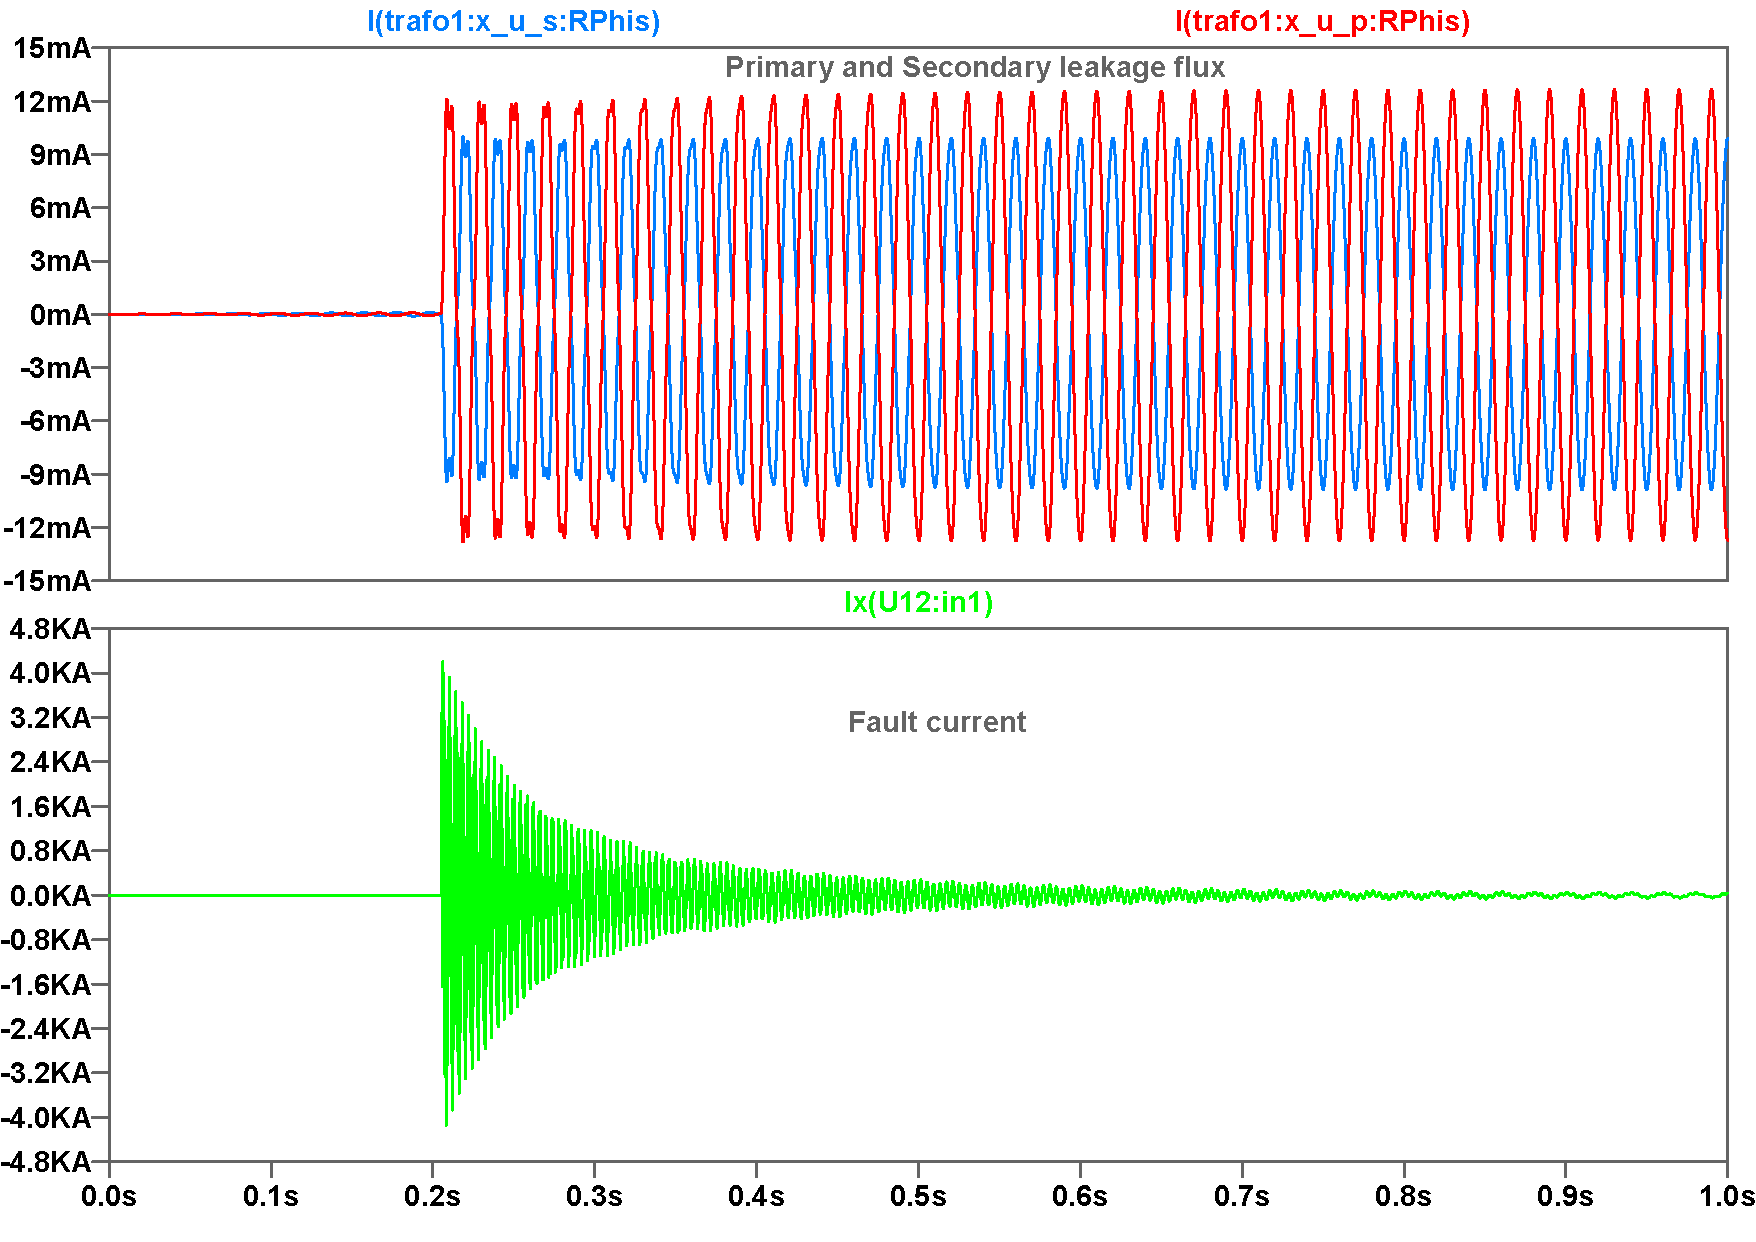
\includegraphics[width=0.90\textwidth]{figures/05_Petersen_earth_faults/Petersen_with_fault_hierarchical_model_TRAN_waveform.pdf}
%	\caption{Petersen with fault TRAN hierarchical model - waveform}
%	\label{fig:Figure3}
%\end{figure}

\begin{figure}[H]
	\centering
	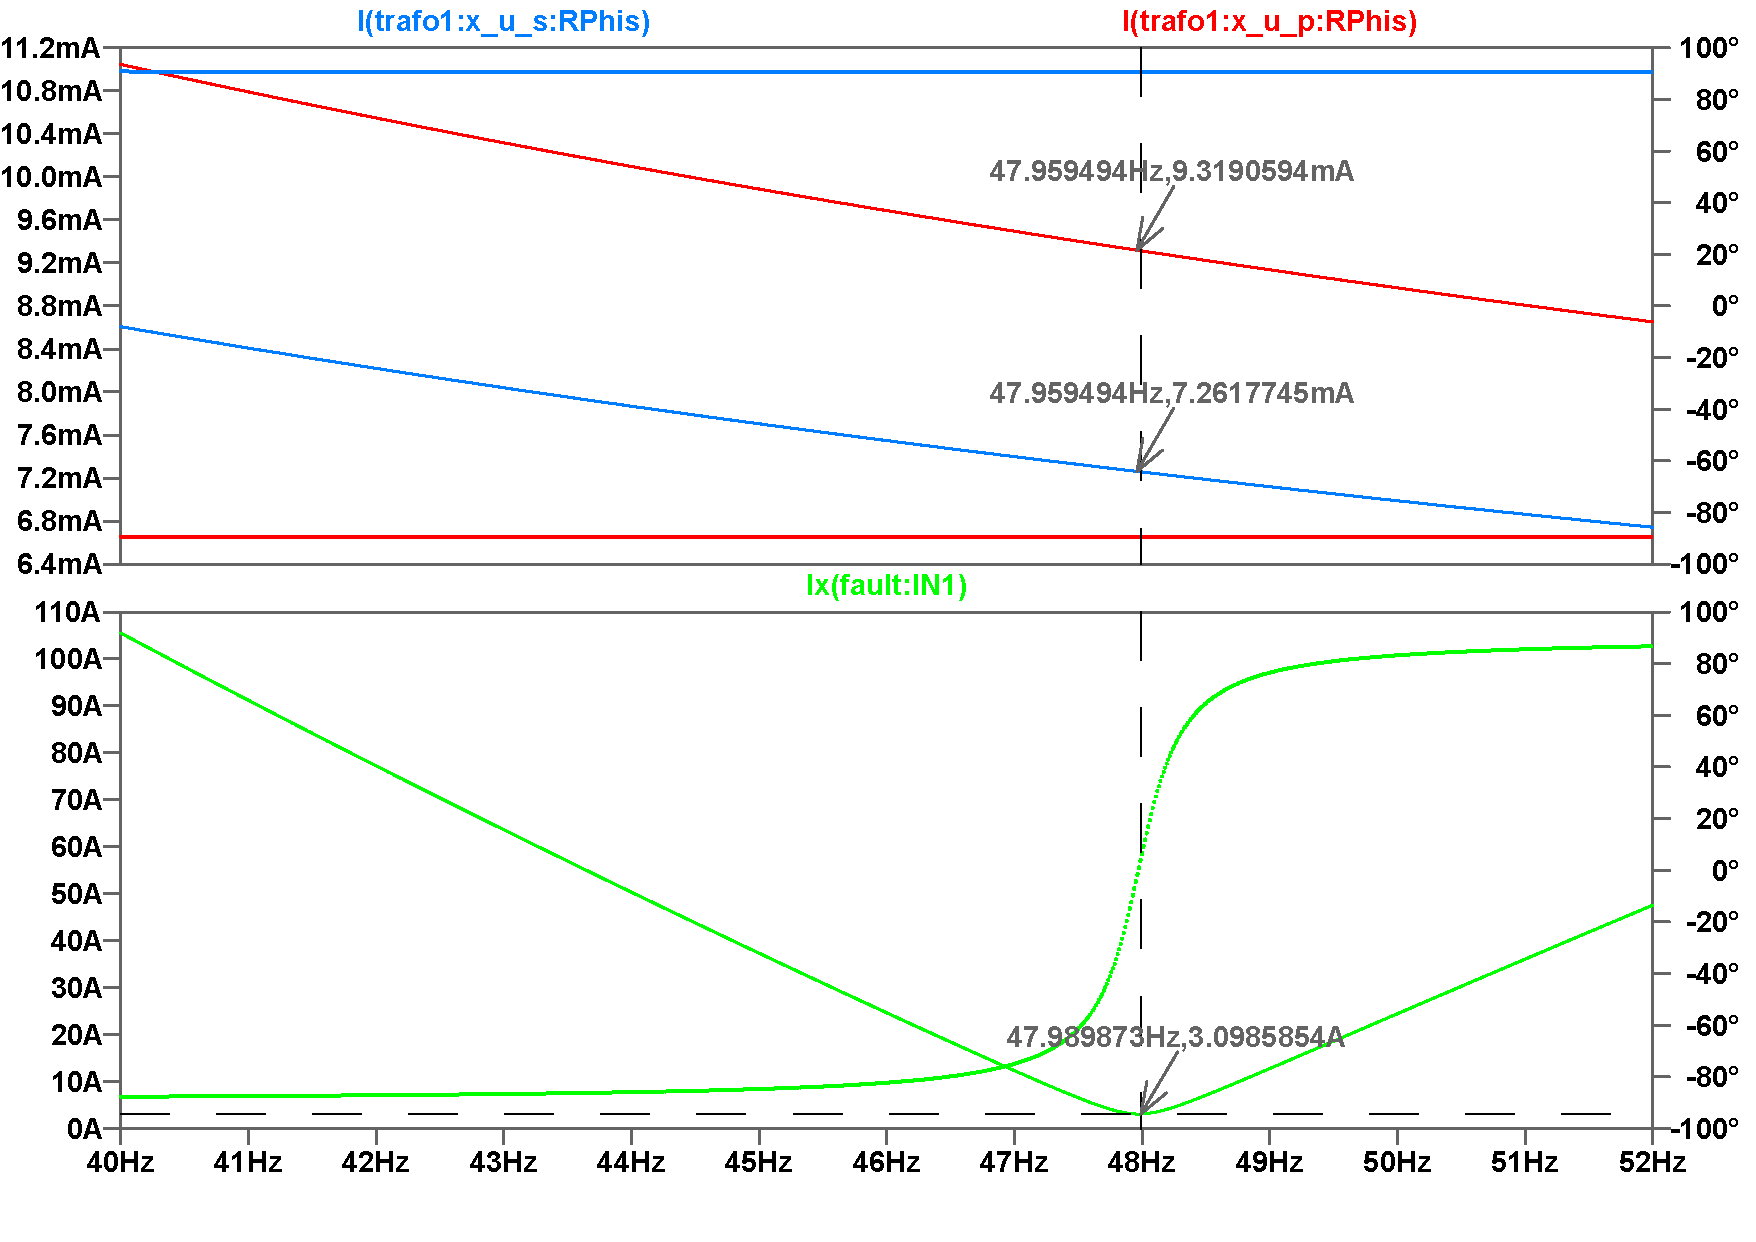
\includegraphics[width=0.90\textwidth]{figures/05_Petersen_earth_faults/Petersen_with_fault_hierarchical_model_AC_waveform.pdf}
	\caption{Petersen with fault AC hierarchical model - waveform}
	\label{fig:Figure4}
\end{figure}

\begin{figure}[H]
	\centering
	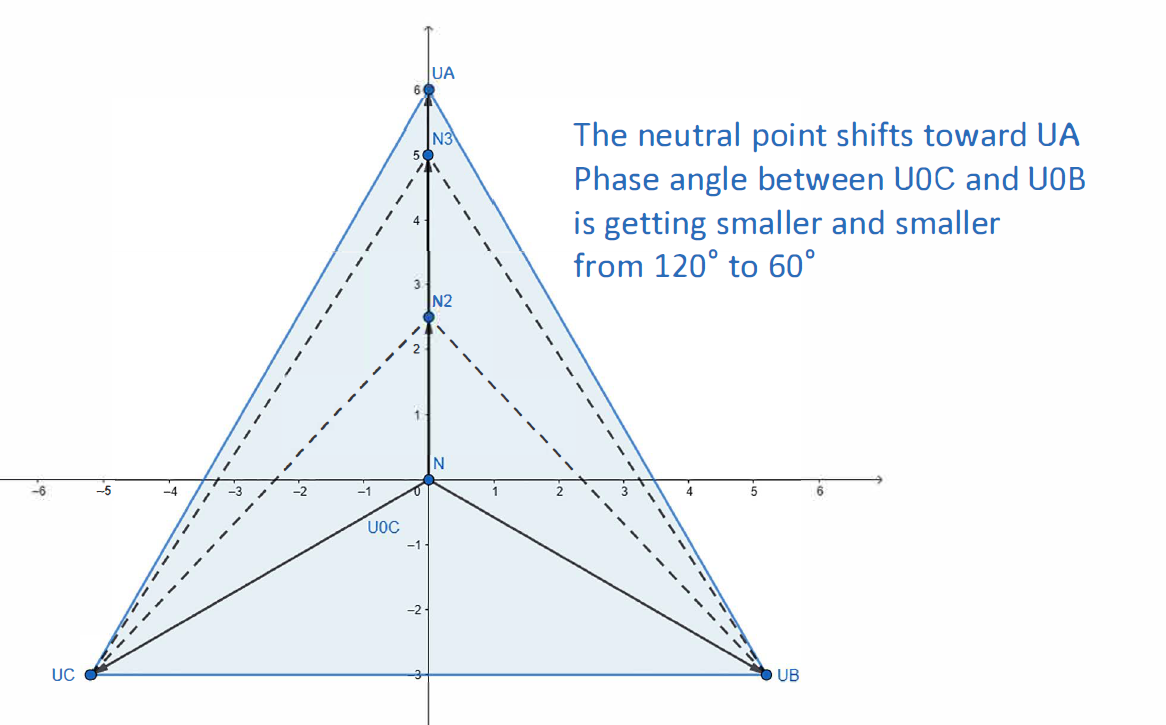
\includegraphics[width=0.90\textwidth]{figures/05_Petersen_earth_faults/Starpoint_Geogebra.png}
	\caption{Principal phase difference between the voltages U0B and U0C in fault case, plotted with GeoGebra - see file Starpoint\_vektor.ggb}
	\label{fig:FigureX}
\end{figure}

%\begin{figure}[H]
%	\centering
%	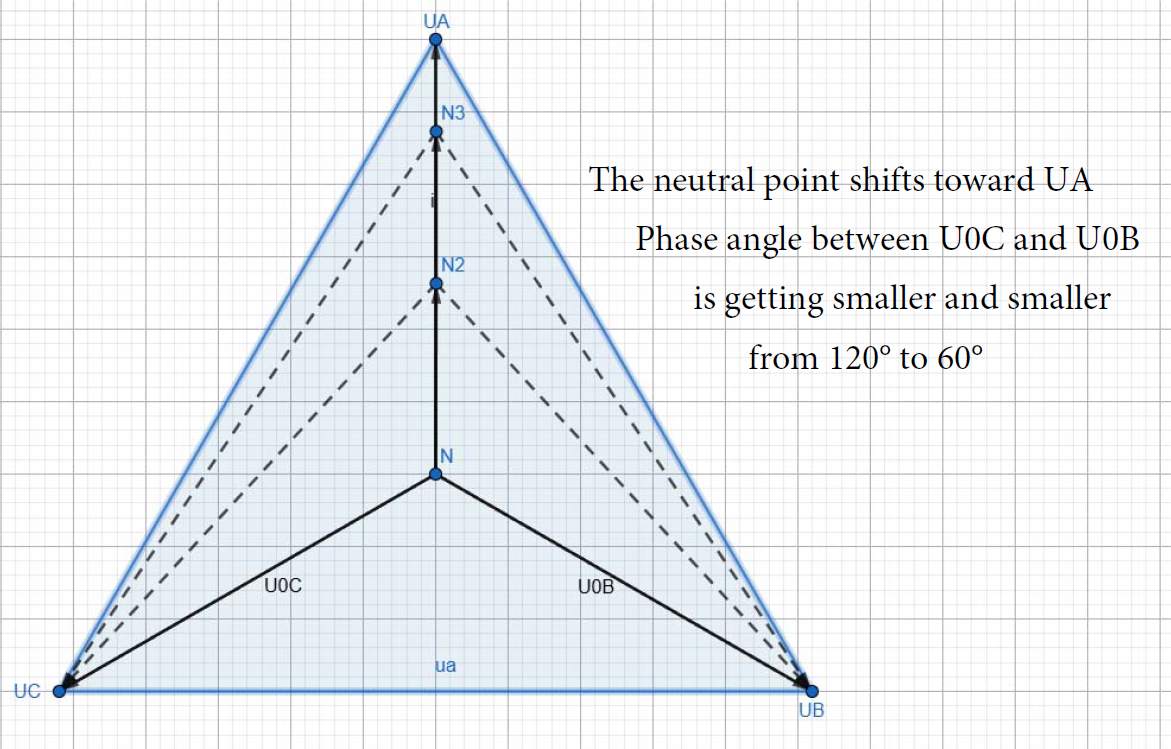
\includegraphics[width=0.90\textwidth]{figures/05_Petersen_earth_faults/Geogebra_Petersen.png}
%	\caption{Phasedifference of the phase voltages U0B,U0C drawn with GeoGebra}
%	\label{fig:FigureX}
%\end{figure}

\begin{figure}[H]
	\centering
	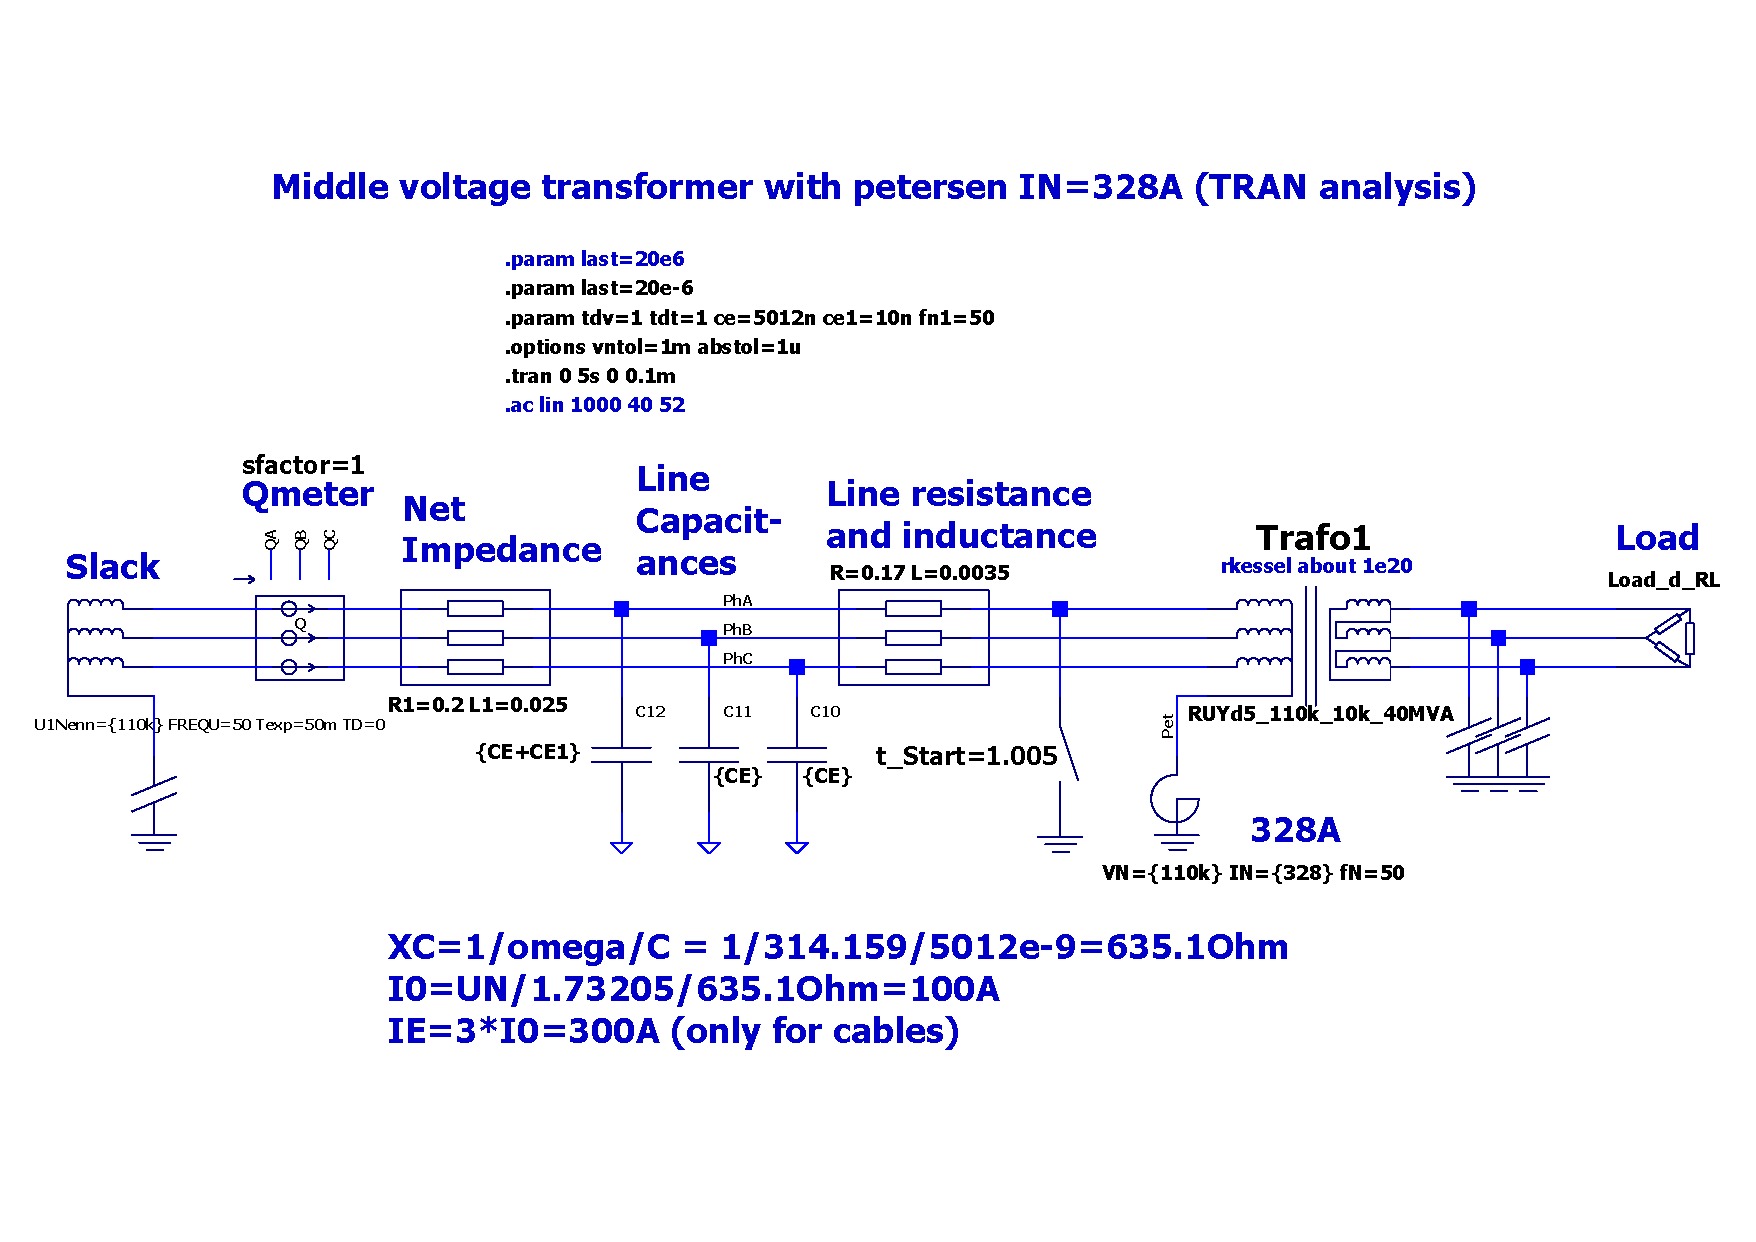
\includegraphics[width=0.90\textwidth]{figures/05_Petersen_earth_faults/Petersen_with_fault_TRAN_schematic.pdf}
	\caption{Petersen with fault TRAN - schematic}
	\label{fig:Figure5a}
\end{figure}

\begin{figure}[H]
	\centering
	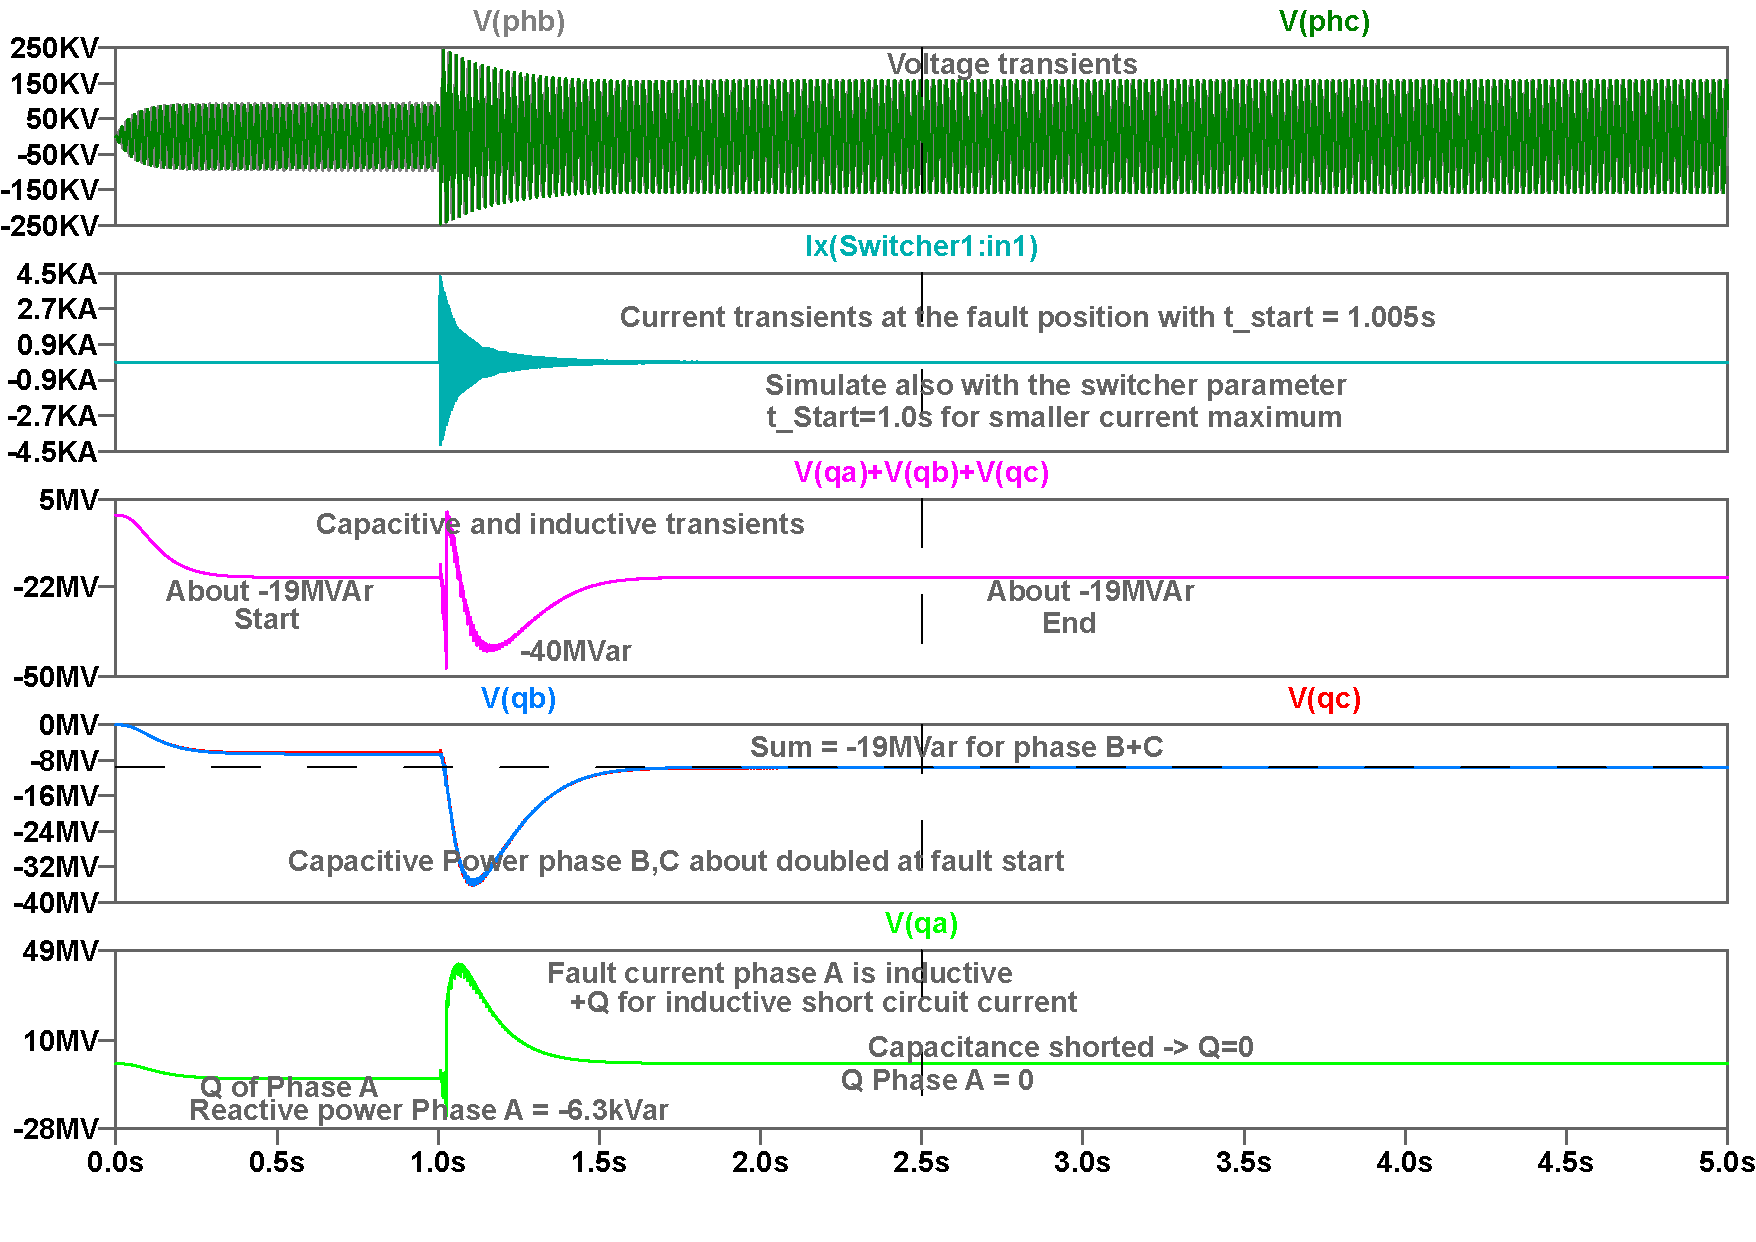
\includegraphics[width=0.90\textwidth]{figures/05_Petersen_earth_faults/Petersen_with_fault_TRAN_waveform.pdf}
	\caption{Petersen with fault TRAN - waveform}
	\label{fig:Figure5}
\end{figure}

\begin{figure}[H]
	\centering
	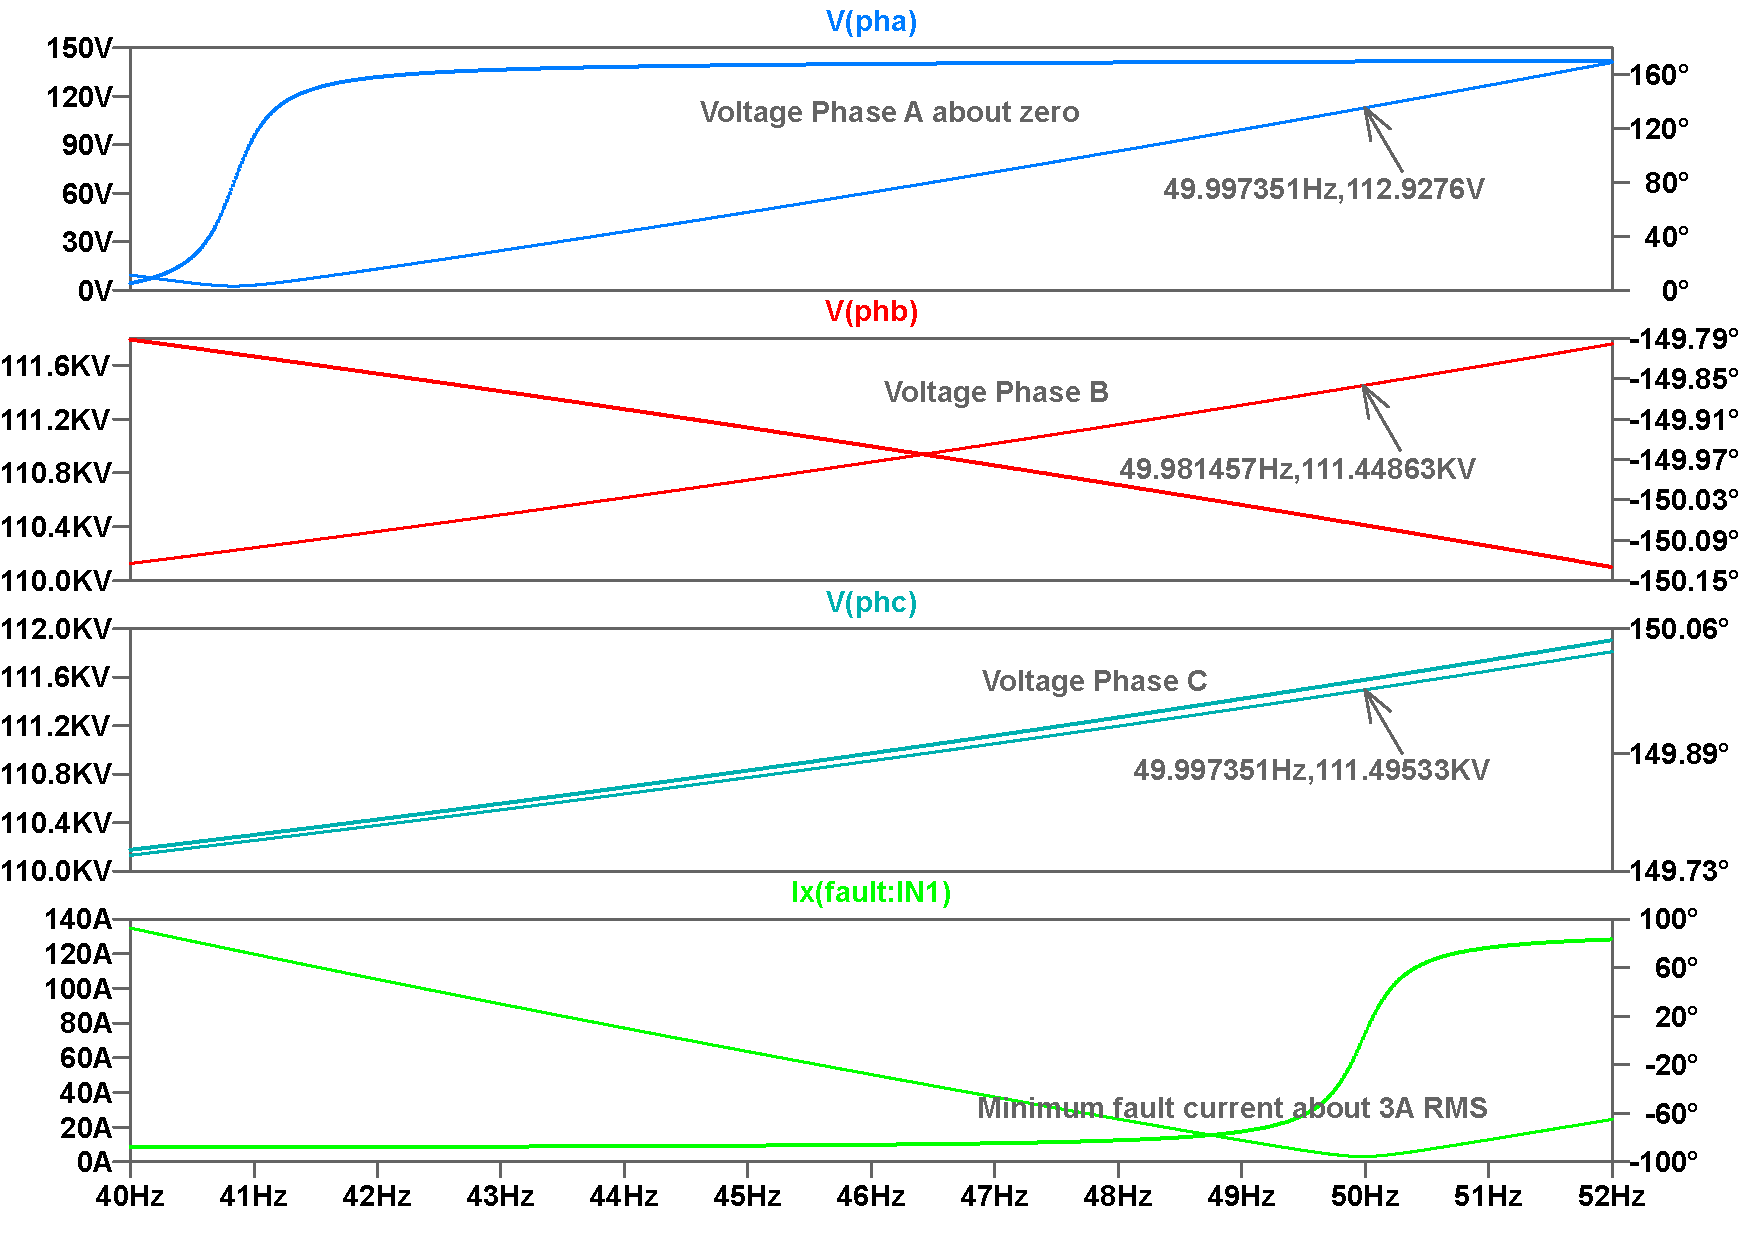
\includegraphics[width=0.90\textwidth]{figures/05_Petersen_earth_faults/Petersen_with_fault_AC_waveform.pdf}
	\caption{Petersen with fault AC - waveform}
	\label{fig:Figure6}
\end{figure}




\begin{figure}[H]
	\centering
	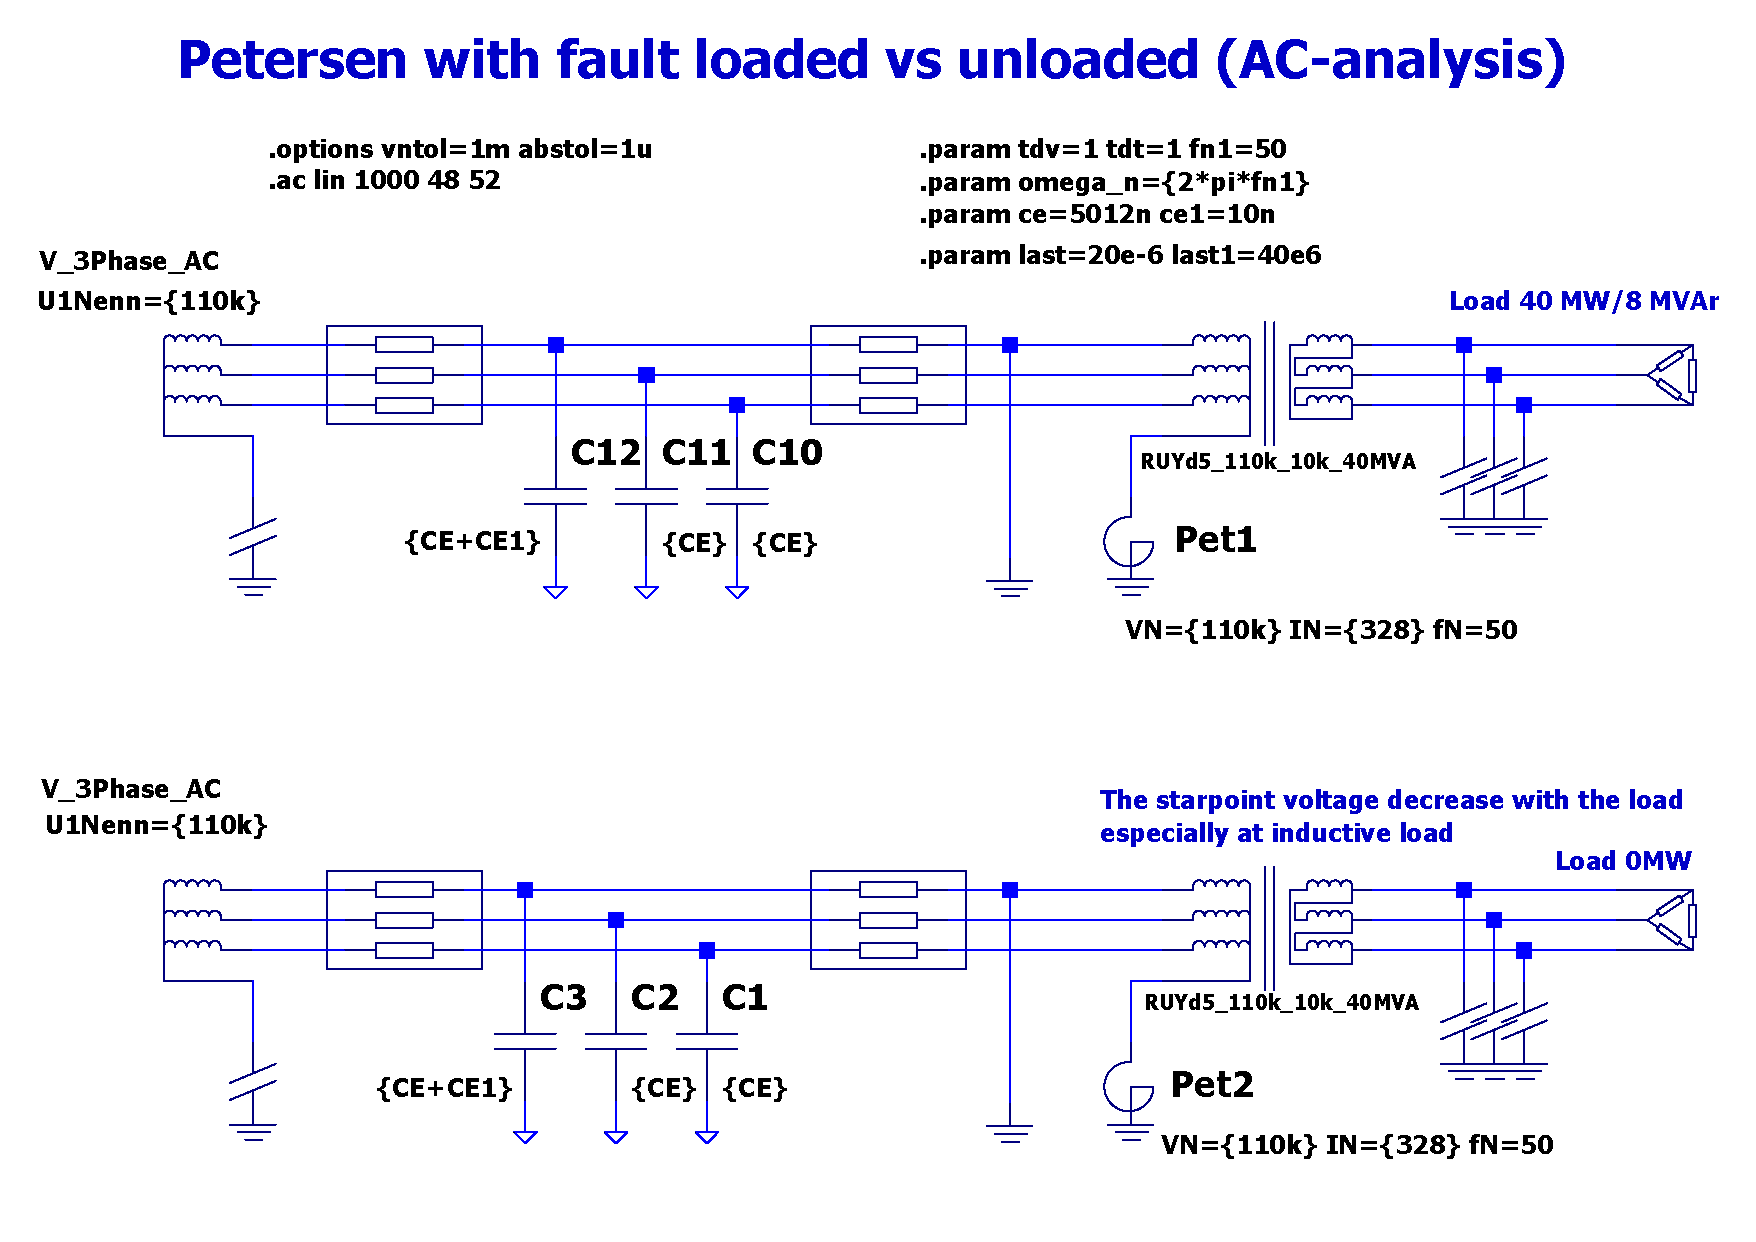
\includegraphics[width=0.90\textwidth]{figures/05_Petersen_earth_faults/Petersen_with_fault_with_load_vs_without_load_AC_schematic.pdf}
	\caption{Petersen with fault and load AC - schematic}
	\label{fig:Figure7a}
\end{figure}

\begin{figure}[H]
	\centering
	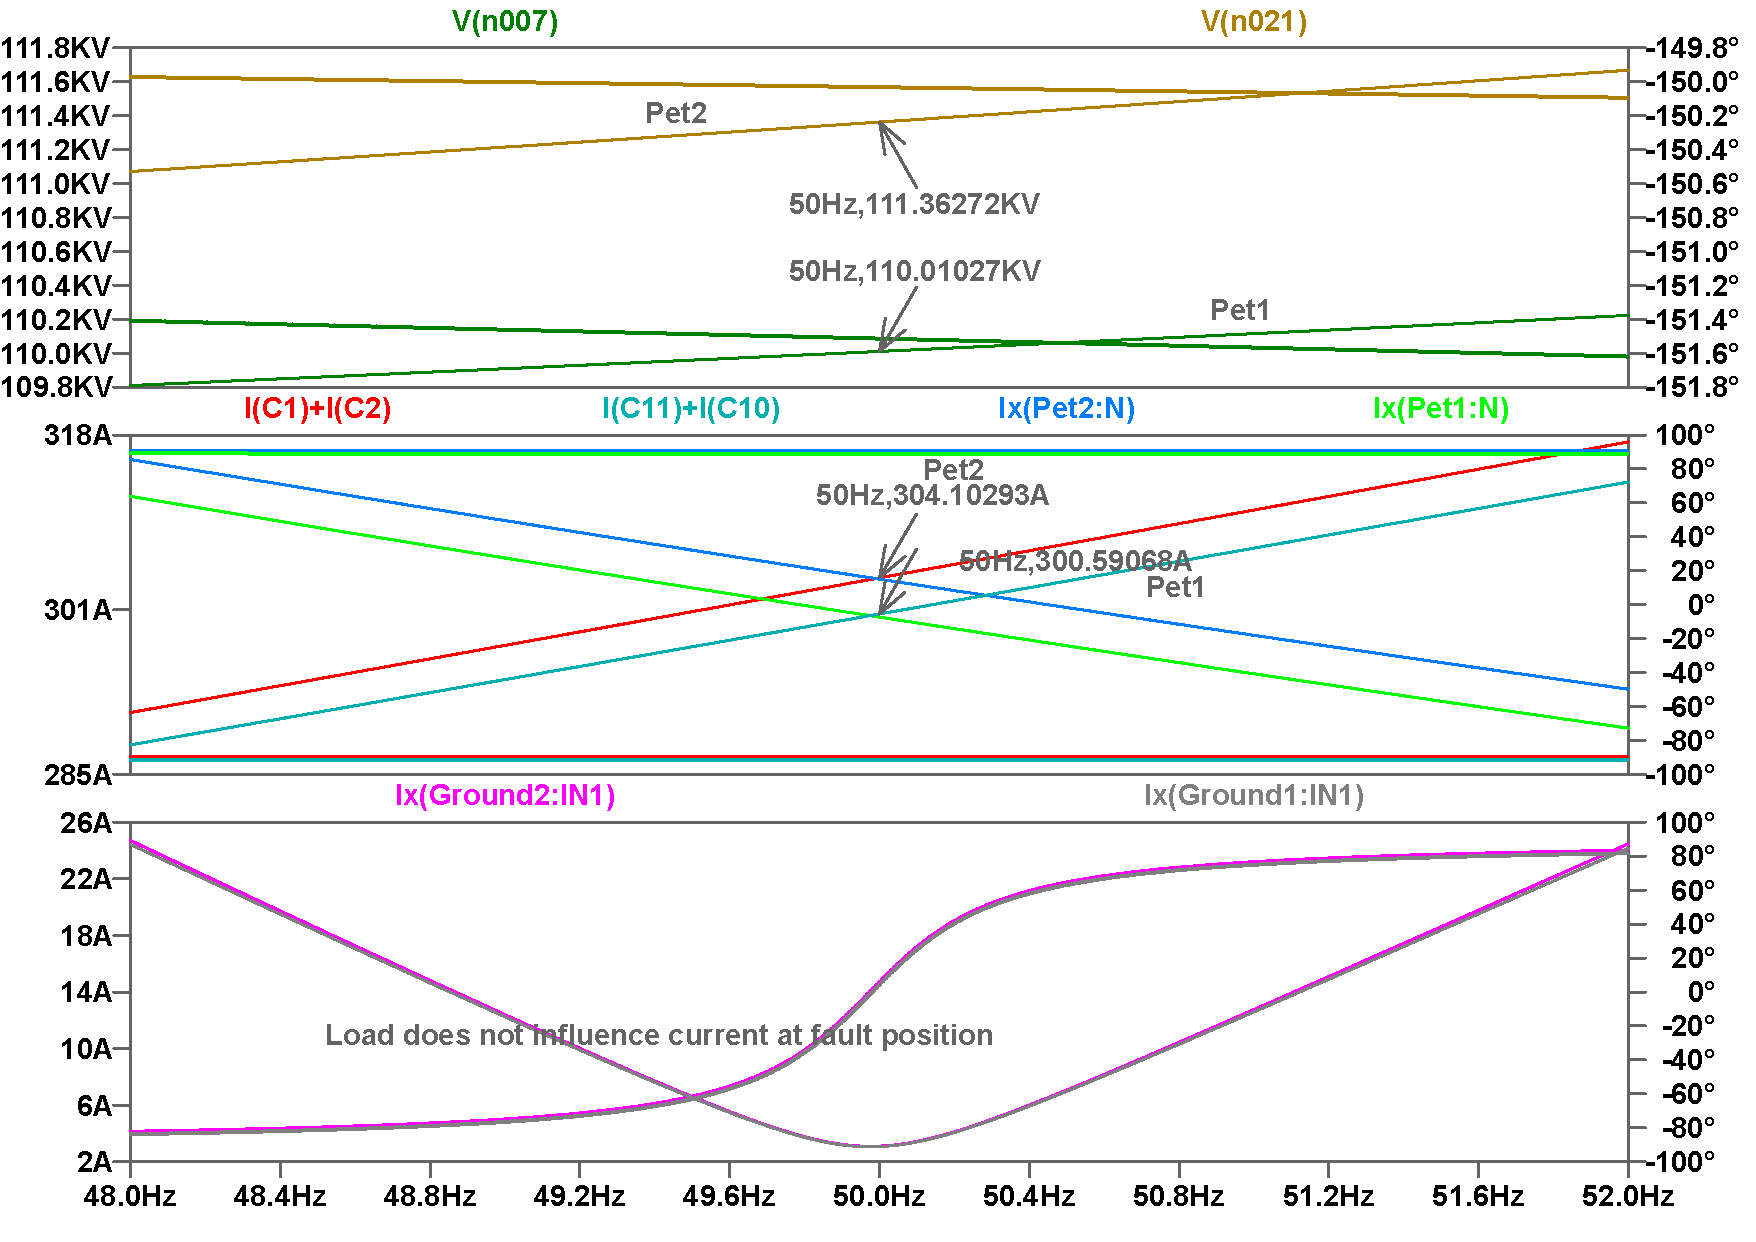
\includegraphics[width=0.90\textwidth]{figures/05_Petersen_earth_faults/Petersen_with_fault_with_load_vs_without_load_AC_waveform.pdf}
	\caption{Petersen with fault and load AC - waveform}
	\label{fig:Figure7}
\end{figure}

\begin{figure}[H]
	\centering
	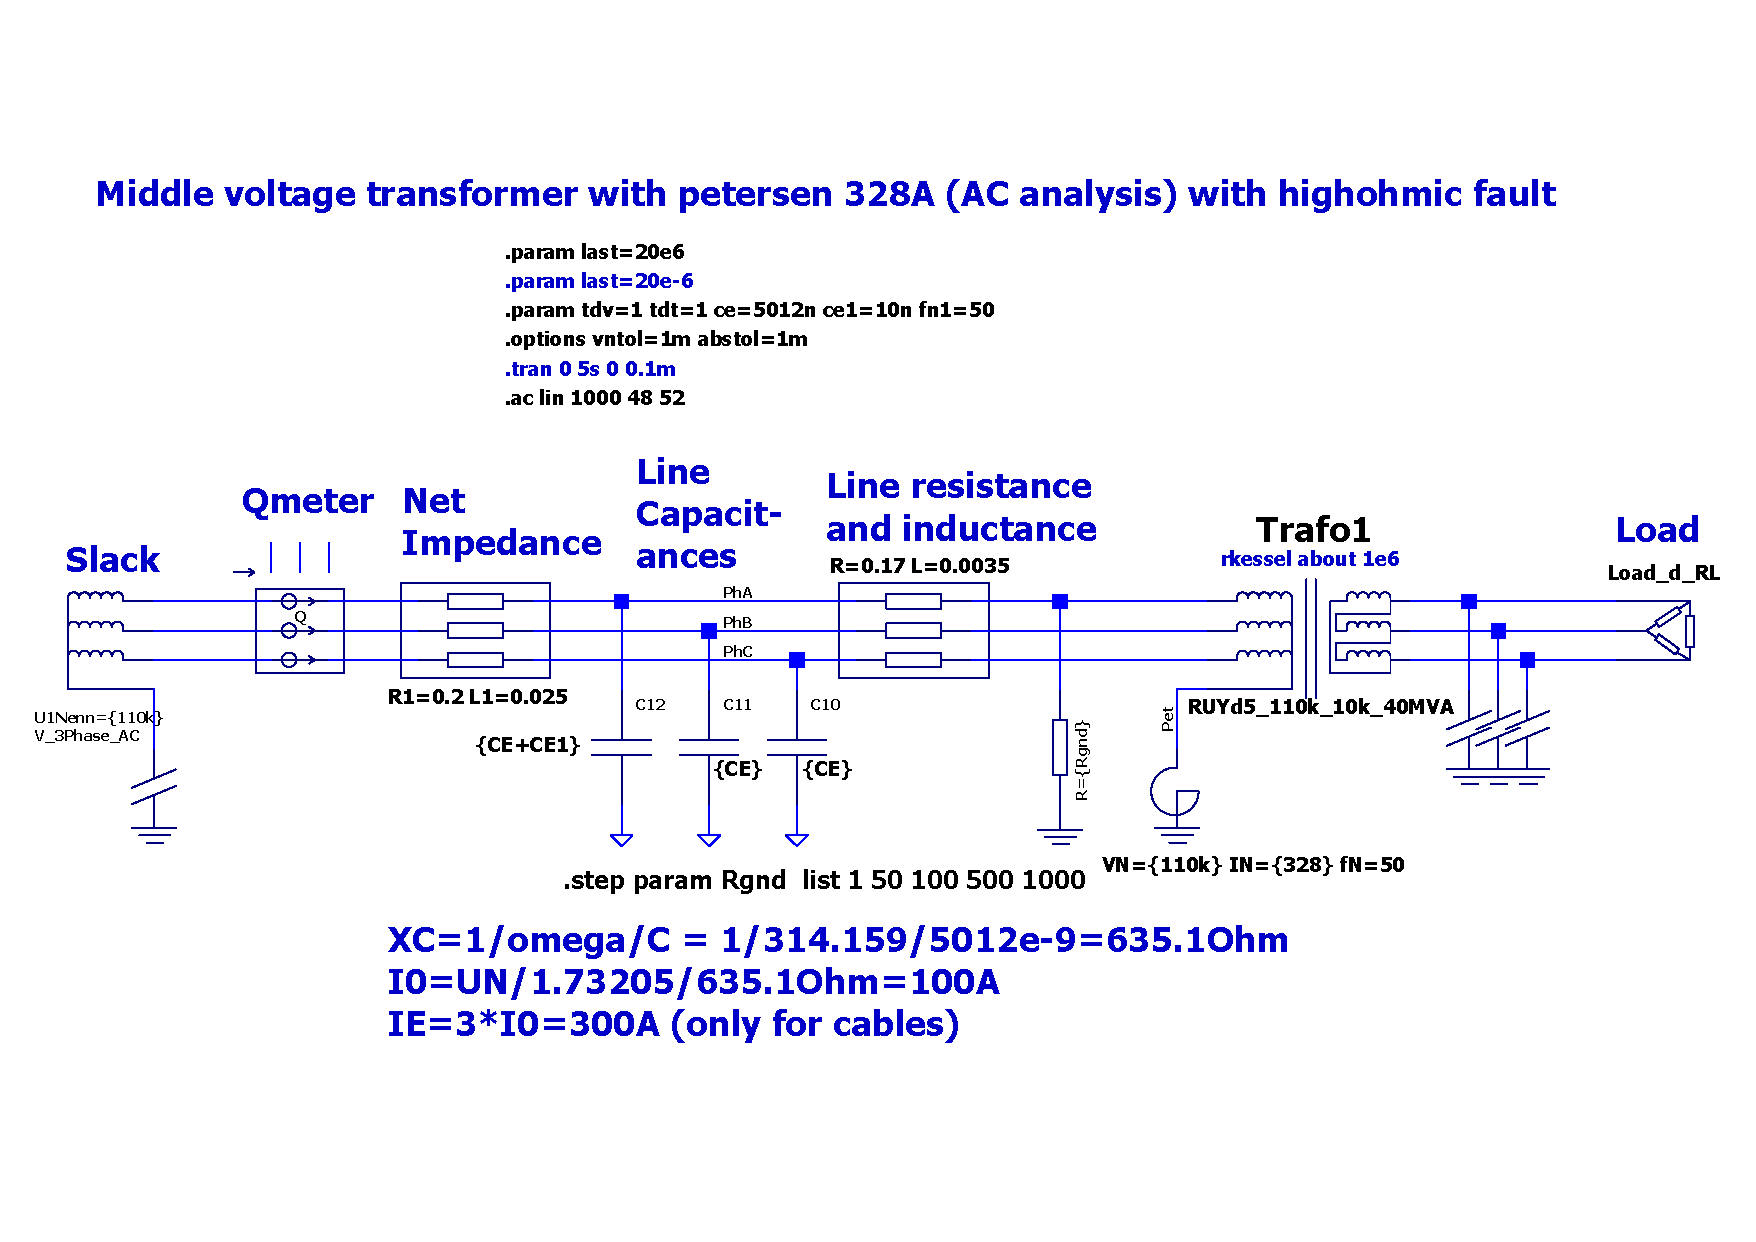
\includegraphics[width=0.90\textwidth]{figures/05_Petersen_earth_faults/Petersen_with_fault_Highohmic_AC_schematic.pdf}
	\caption{Petersen with high-resistance earth fault fault AC - schematic}
	\label{fig:Figure8a}
\end{figure}

\begin{figure}[H]
	\centering
	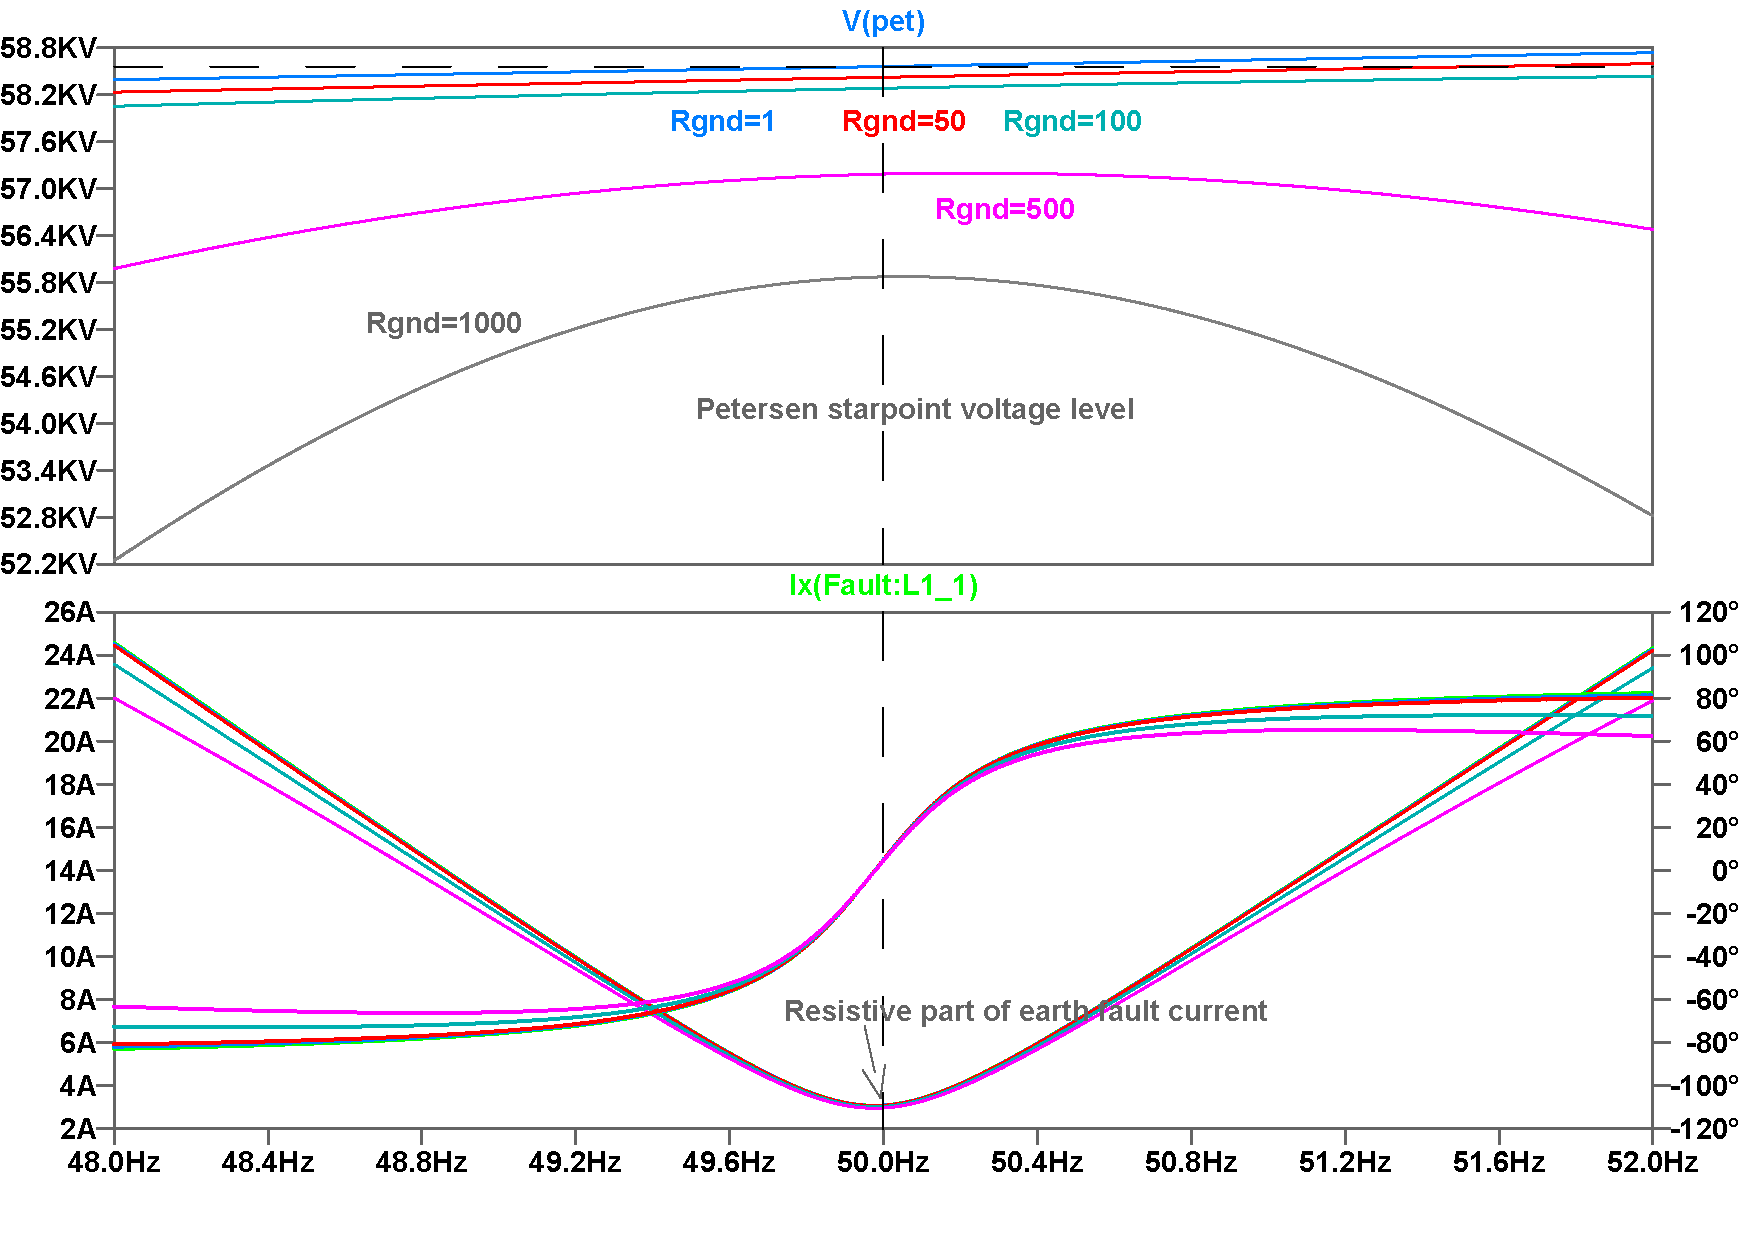
\includegraphics[width=0.90\textwidth]{figures/05_Petersen_earth_faults/Petersen_with_fault_Highohmic_AC_waveform.pdf}
	\caption{Petersen with high-resistance earth fault fault AC - waveform}
	\label{fig:Figure8}
\end{figure}

\begin{figure}[H]
	\centering
	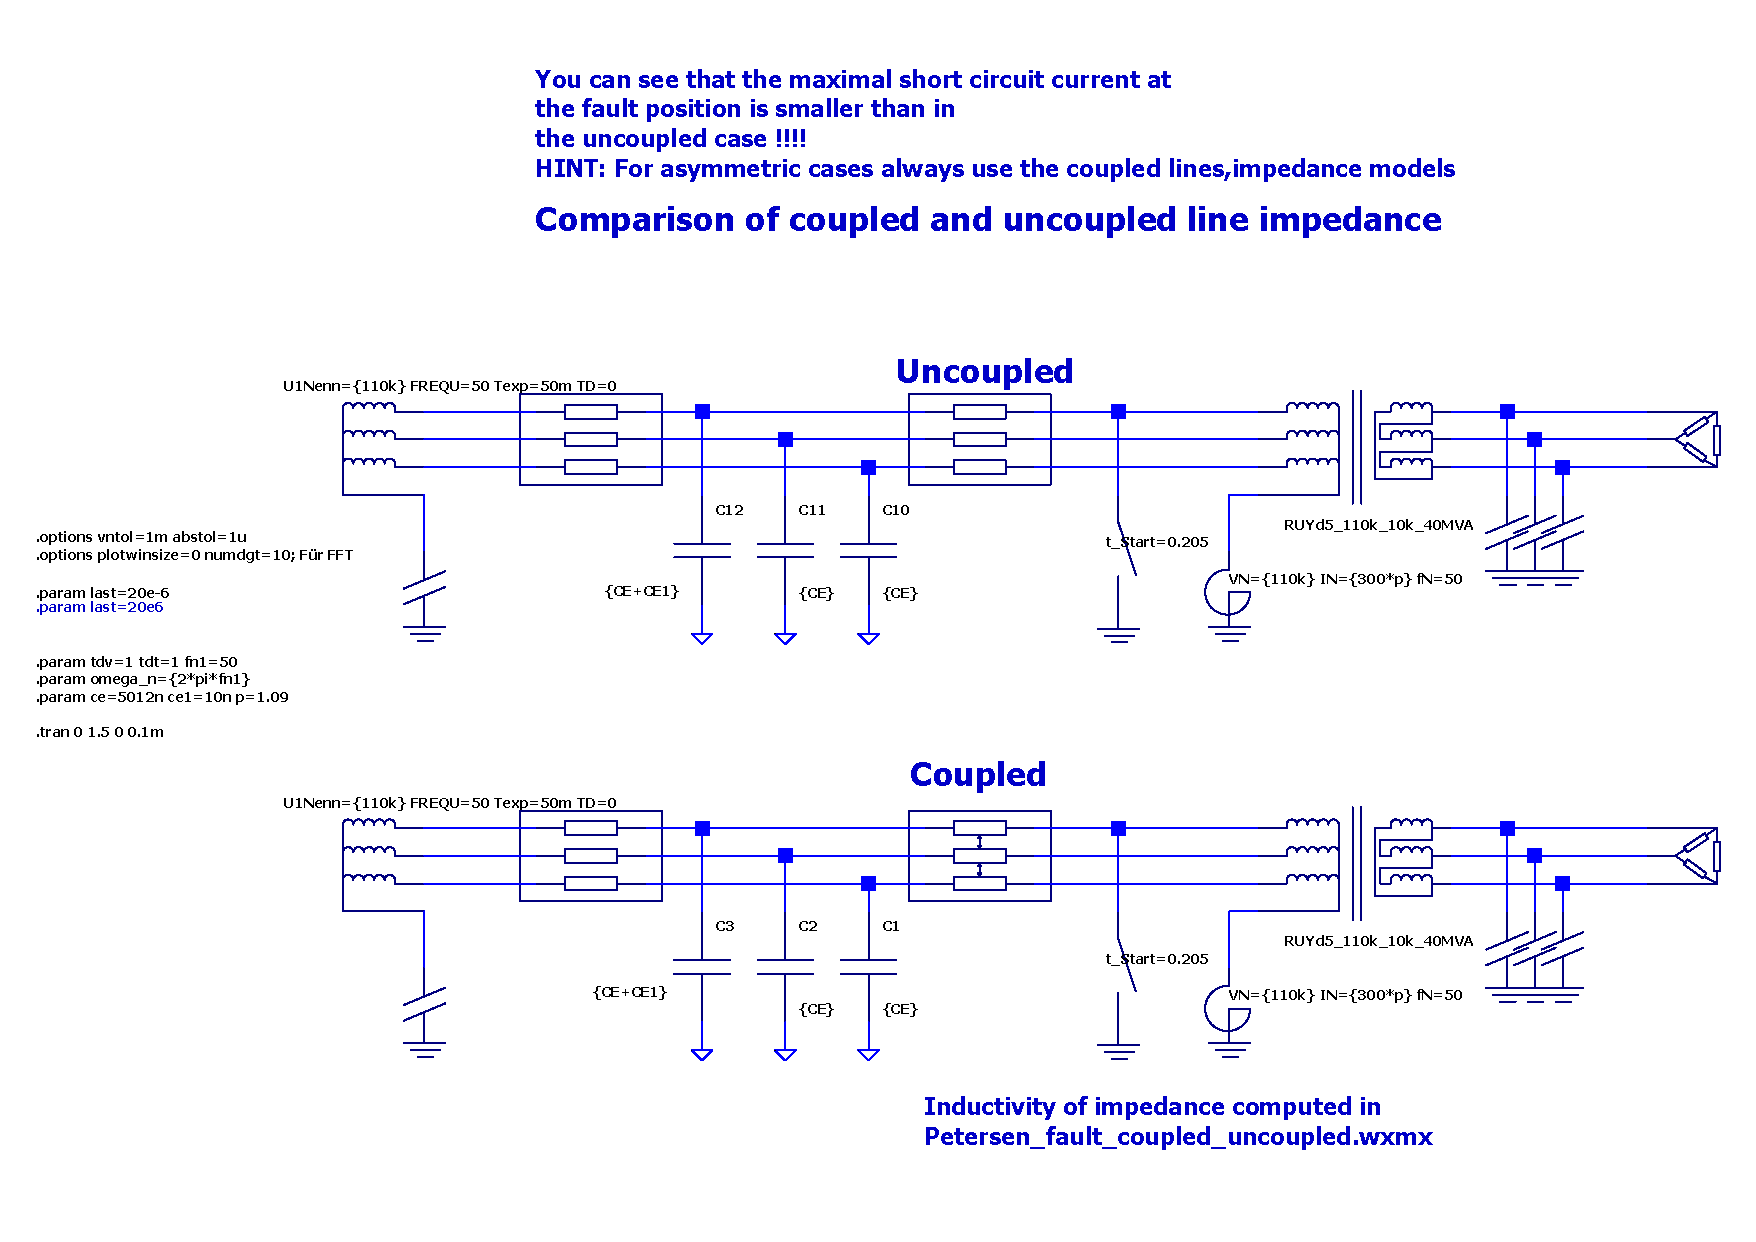
\includegraphics[width=0.90\textwidth]{figures/05_Petersen_earth_faults/Petersen_fault_coupled_uncoupled_schematic.pdf}
	\caption{Petersen with coupled and uncoupled line impedance - schematic}
	\label{fig:Figure9a}
\end{figure}

\begin{figure}[H]
	\centering
	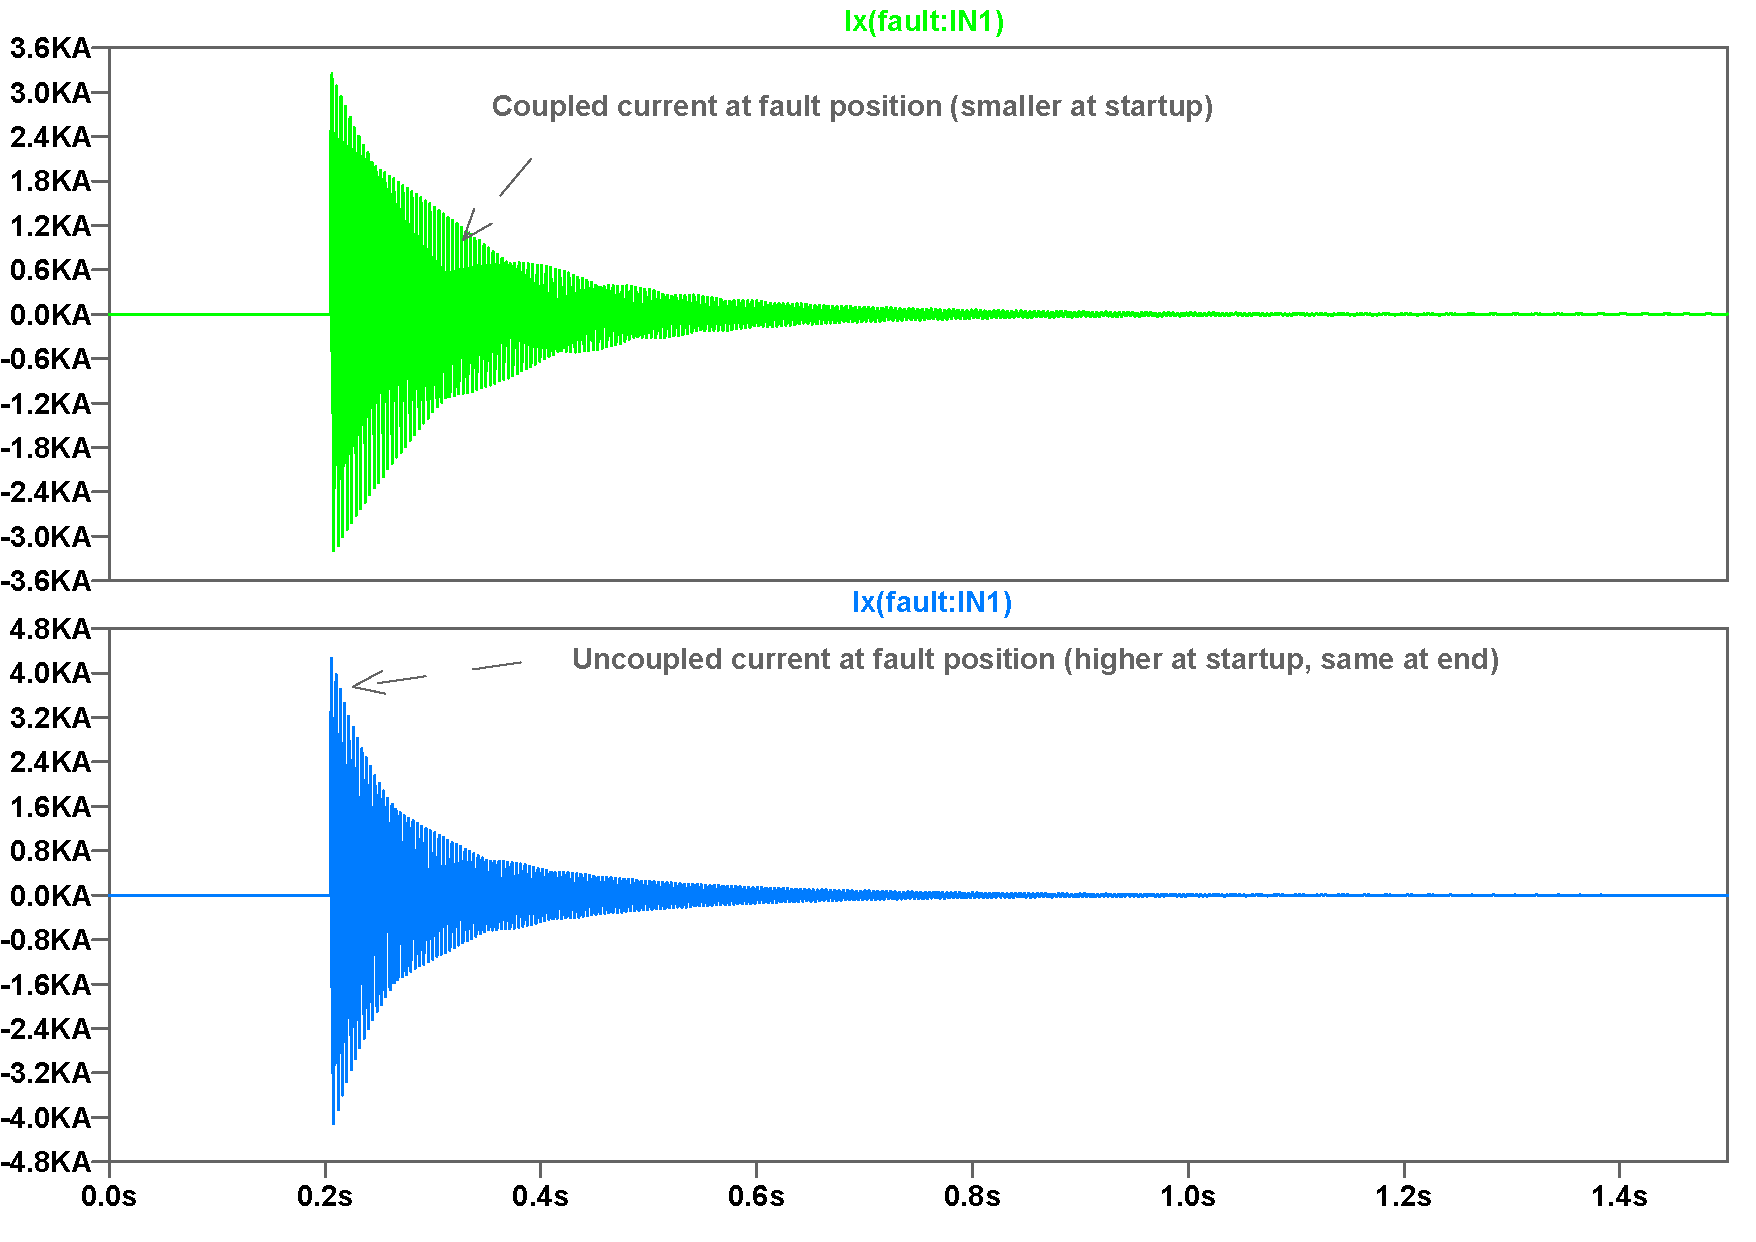
\includegraphics[width=0.90\textwidth]{figures/05_Petersen_earth_faults/Petersen_fault_coupled_uncoupled_waveform.pdf}
	\caption{Petersen with coupled and uncoupled line impedance - waveform}
	\label{fig:Figure9}
\end{figure}

\begin{figure}[H]
	\centering
	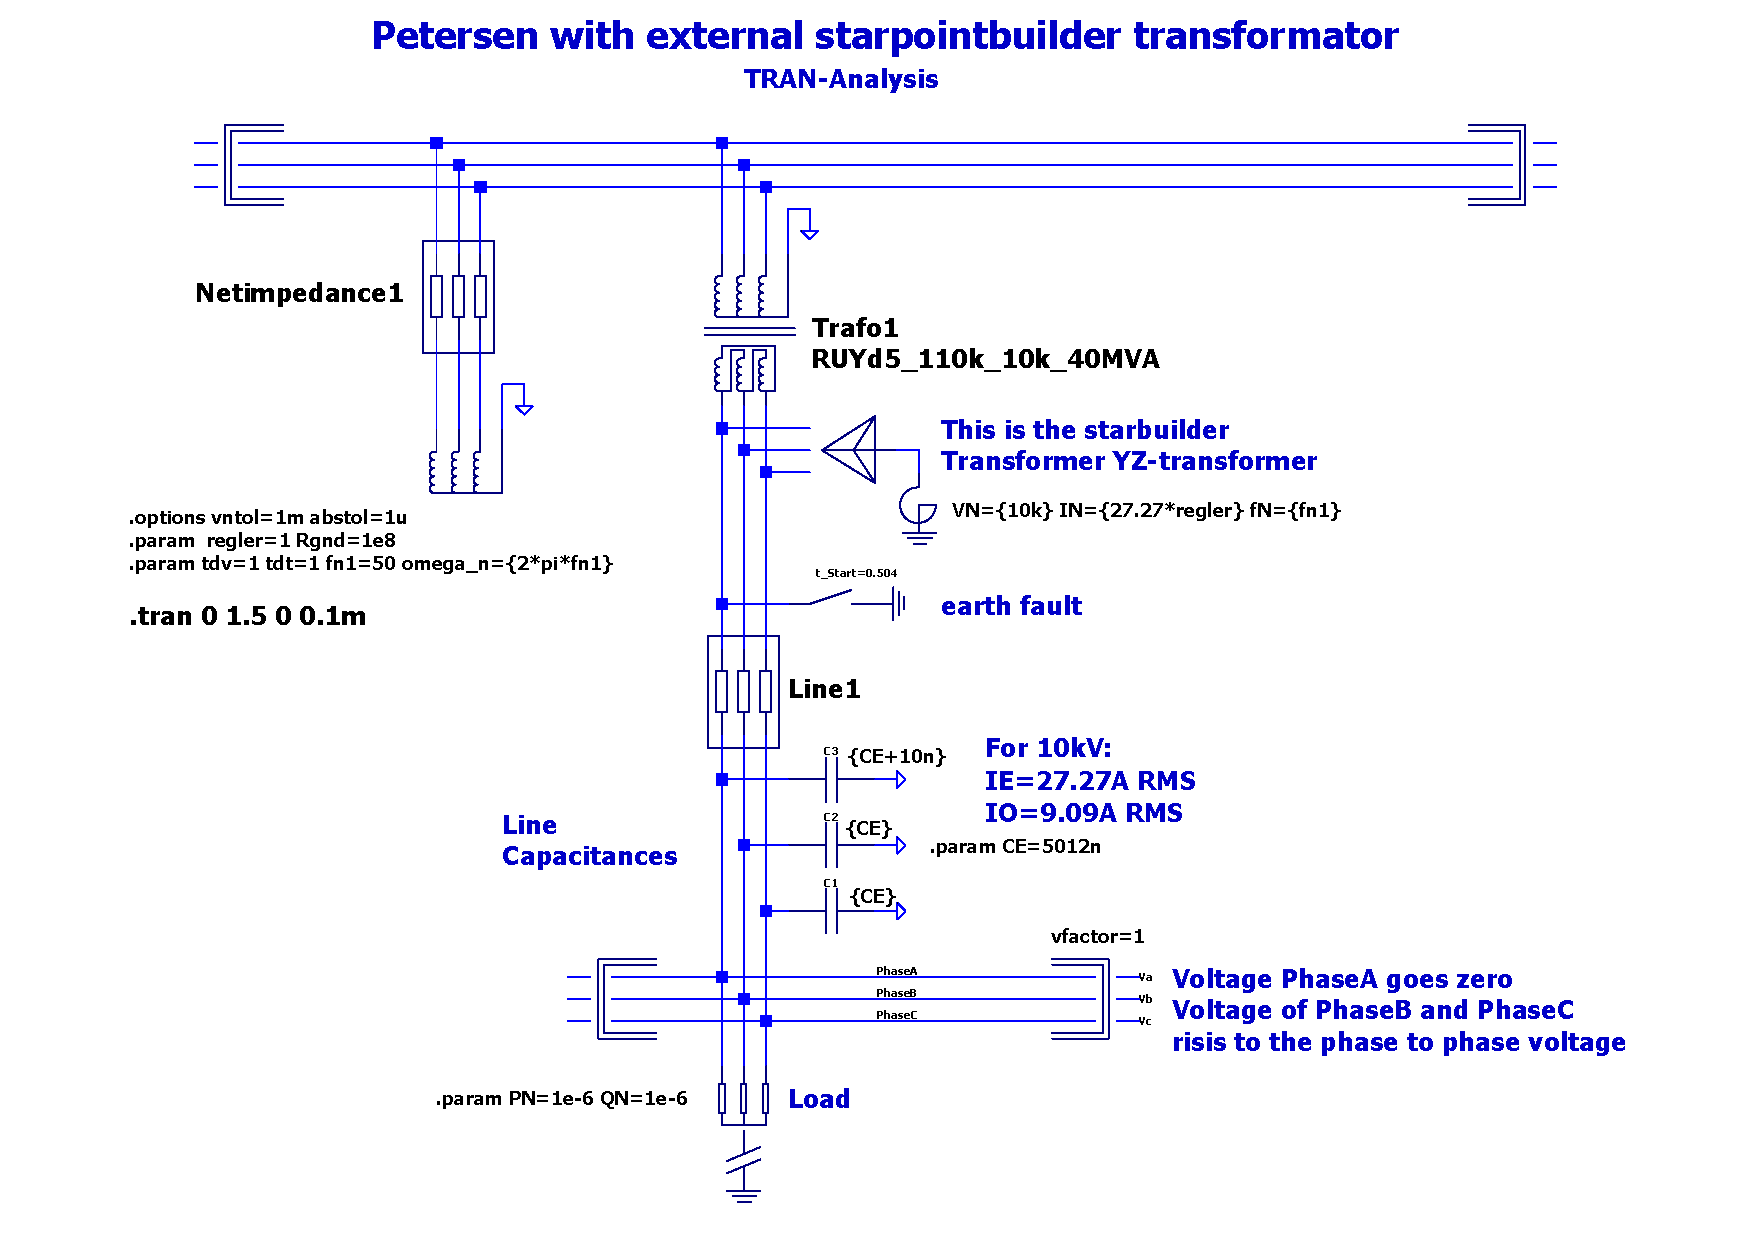
\includegraphics[width=0.90\textwidth]{figures/05_Petersen_earth_faults/Petersen_trafo_gnd_TRAN_schematic.pdf}
	\caption{Petersen without fault and external grounding transformer TRAN - schematic}
	\label{fig:Figure10a}
\end{figure}

\begin{figure}[H]
	\centering
	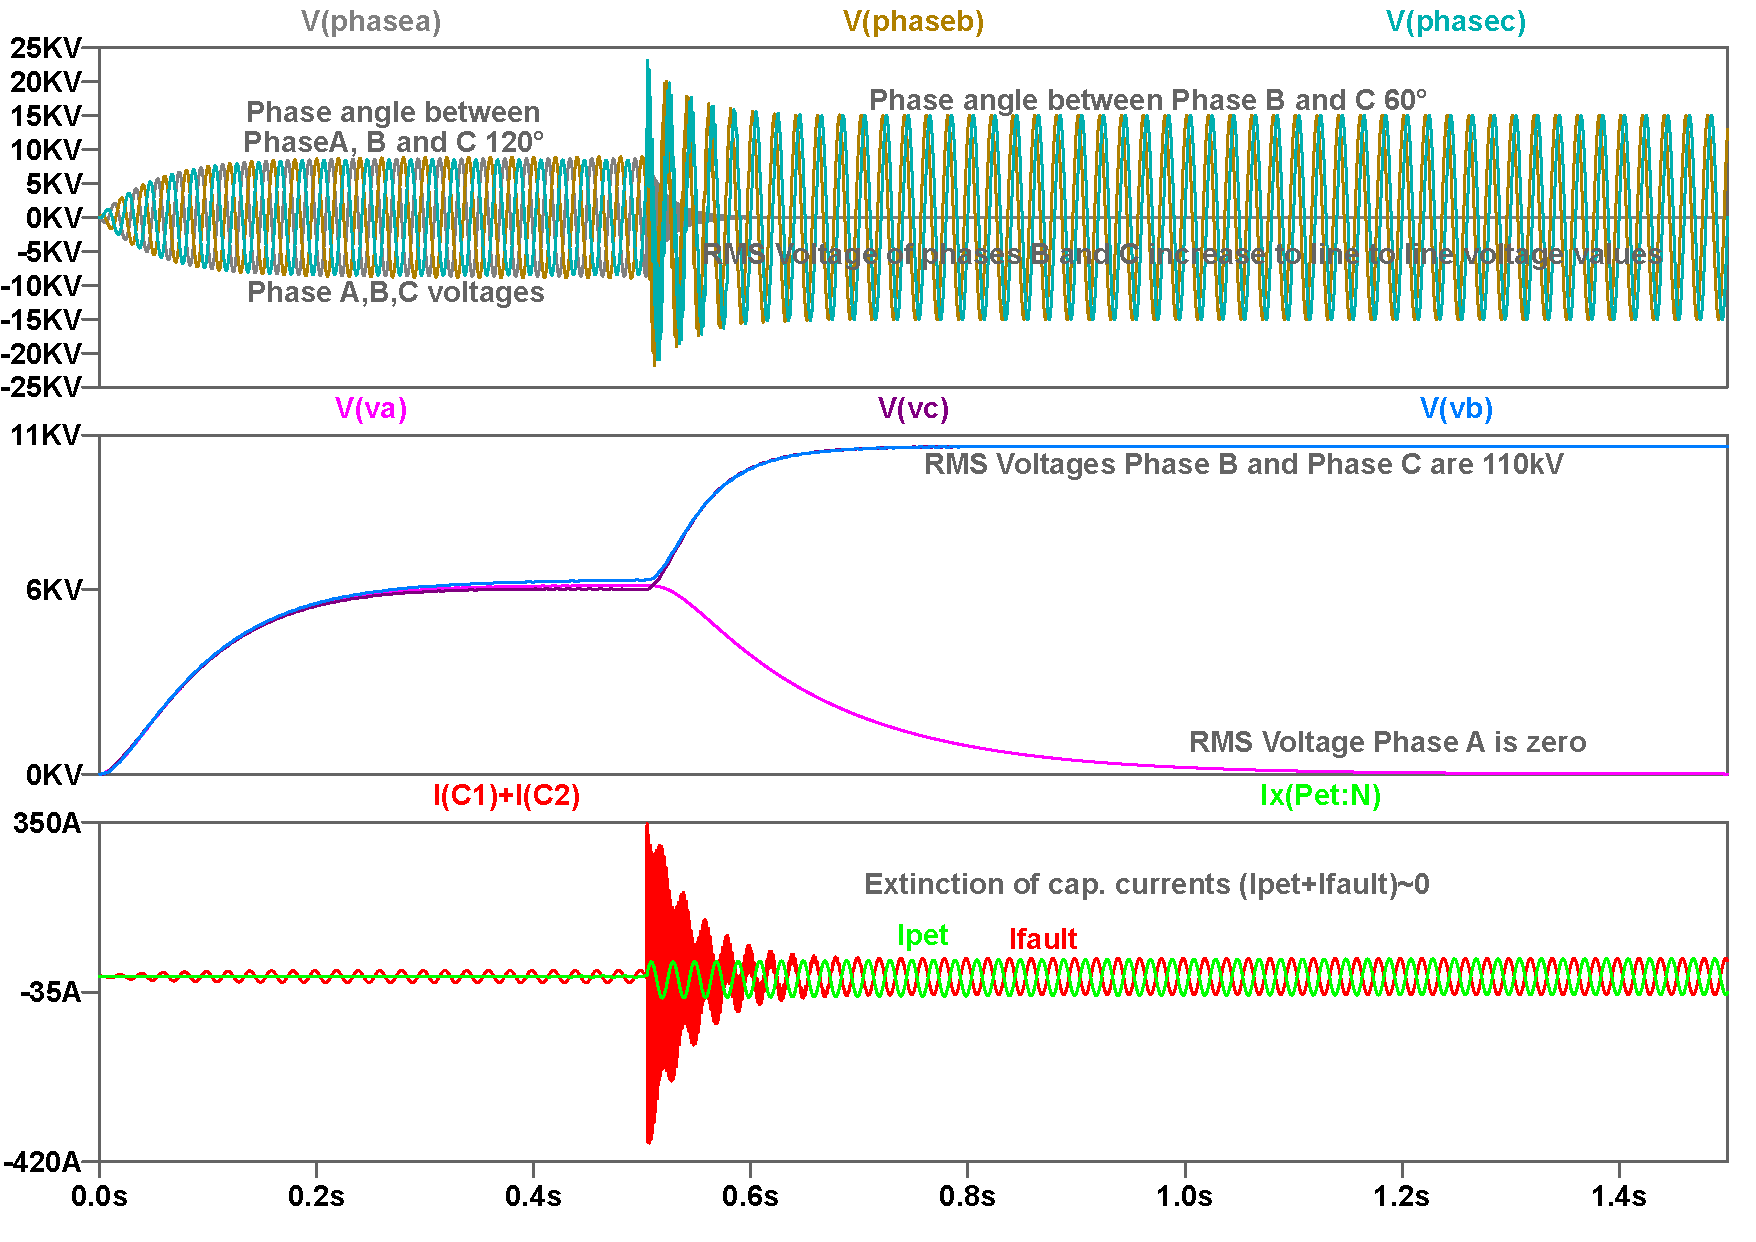
\includegraphics[width=0.90\textwidth]{figures/05_Petersen_earth_faults/Petersen_trafo_gnd_TRAN_waveform.pdf}
	\caption{Petersen without fault and external grounding transformer TRAN - waveform}
	\label{fig:Figure10}
\end{figure}

\begin{figure}[H]
	\centering
	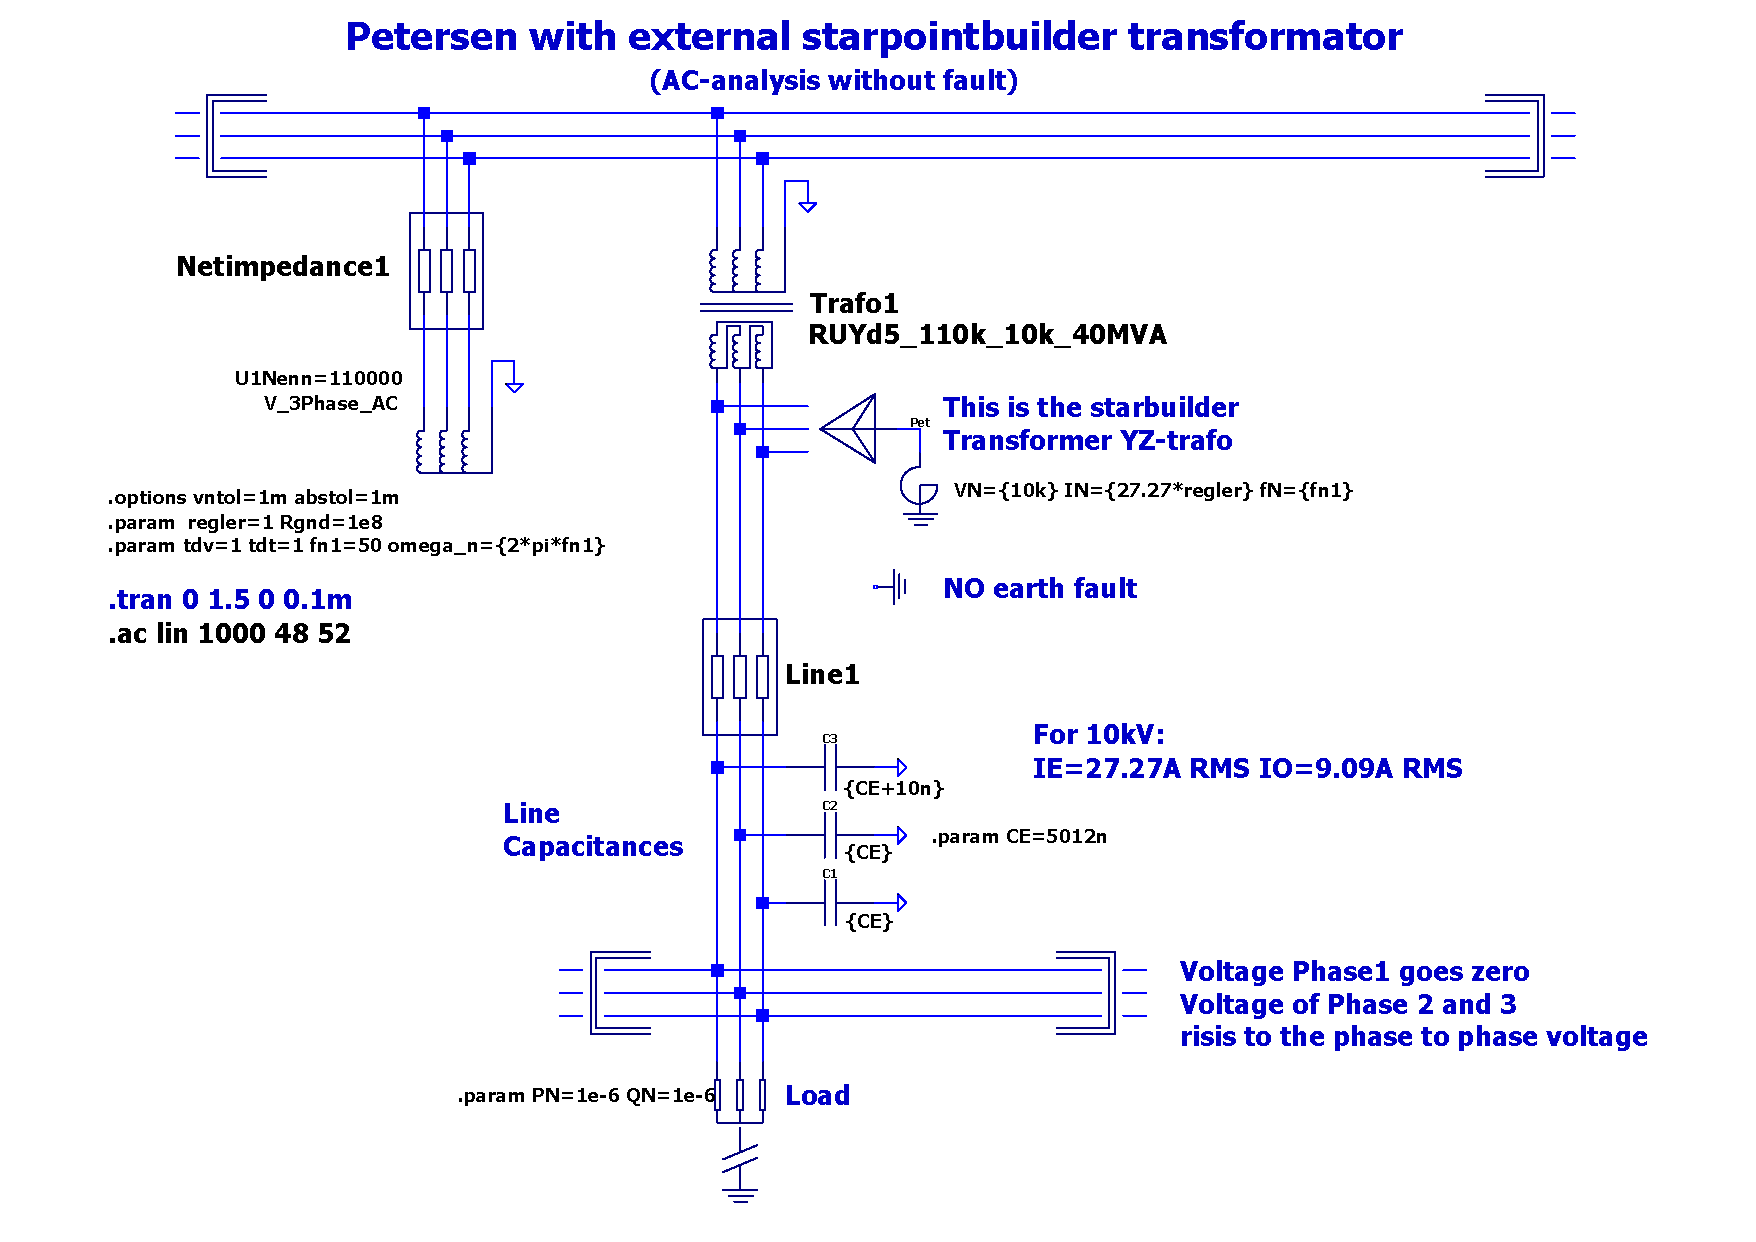
\includegraphics[width=0.90\textwidth]{figures/05_Petersen_earth_faults/Petersen_trafo_gnd_AC_no_fault_schematic.pdf}
	\caption{Petersen without fault and external grounding transformer AC - schematic}
	\label{fig:Figure11a}
\end{figure}

\begin{figure}[H]
	\centering
	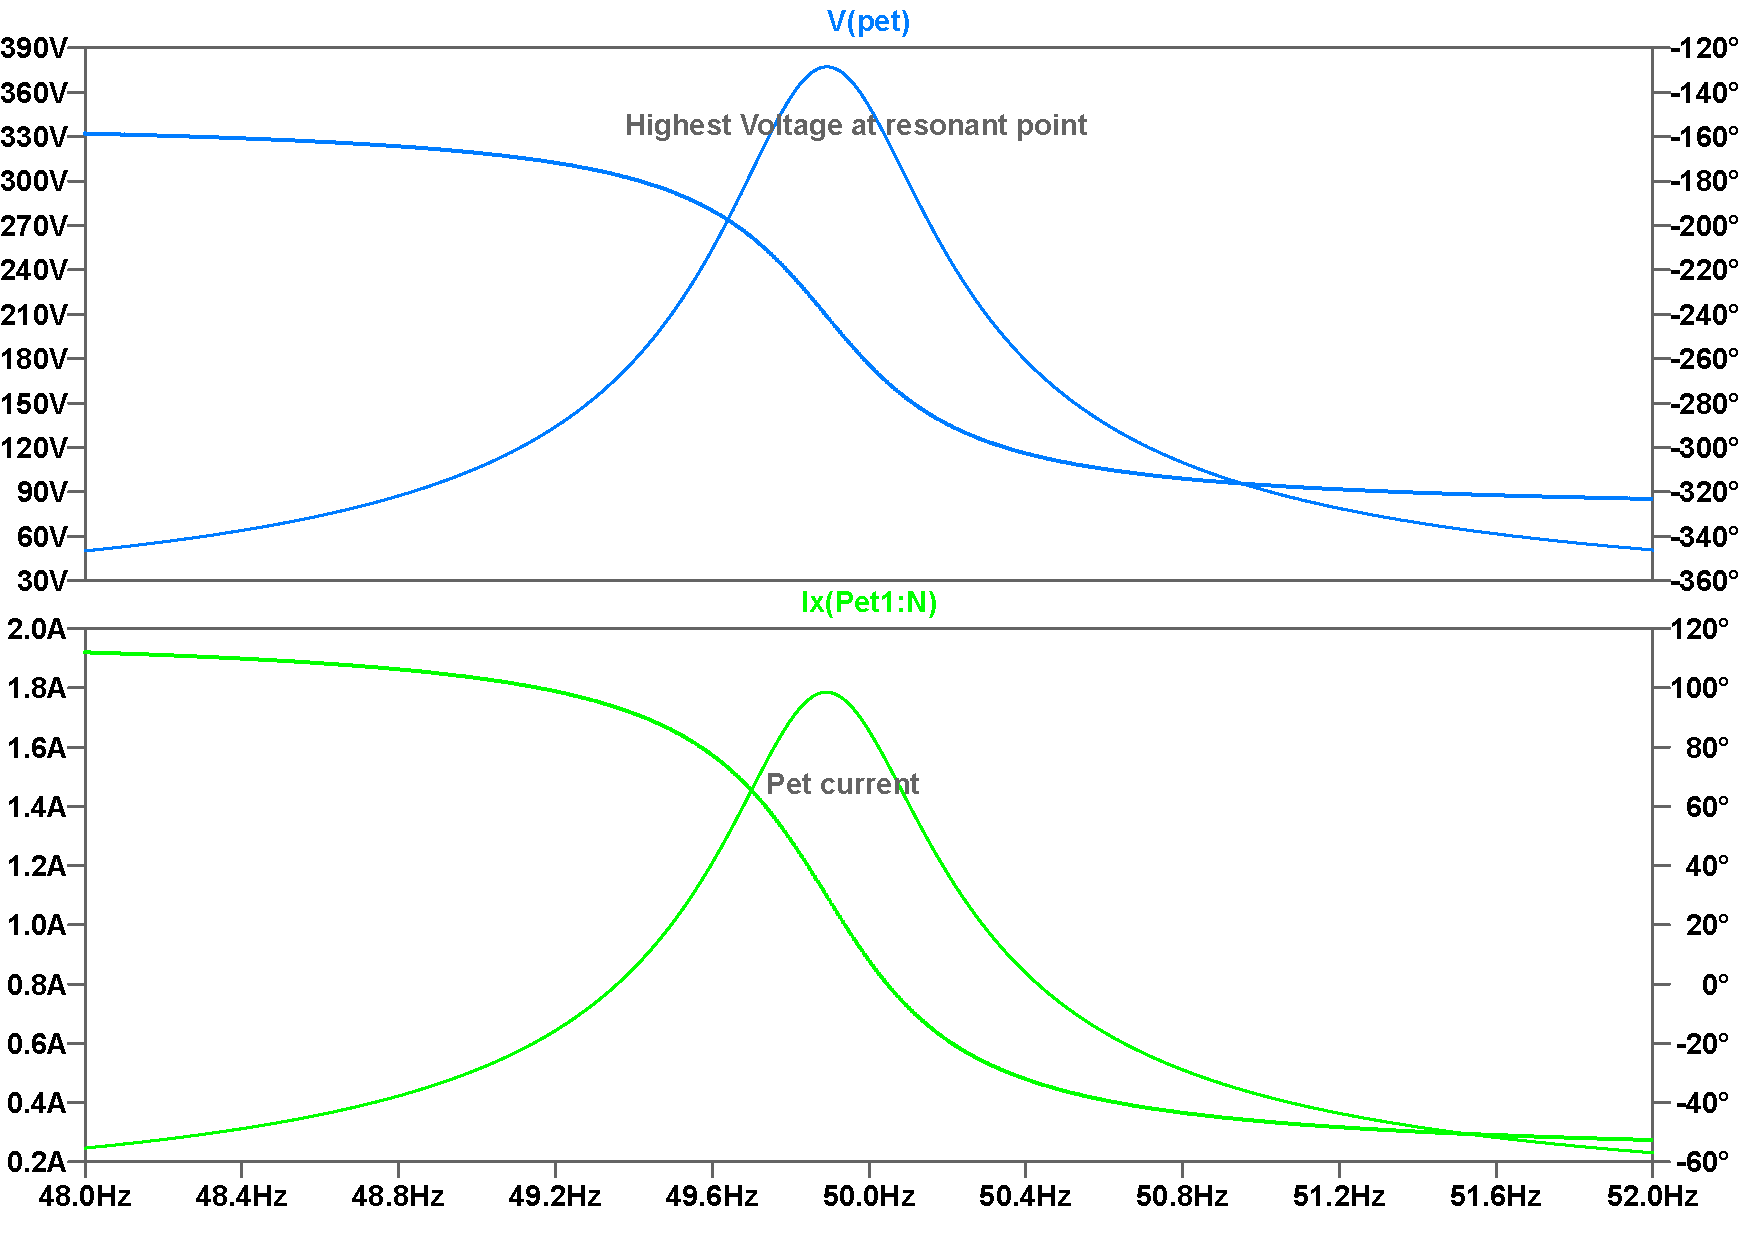
\includegraphics[width=0.90\textwidth]{figures/05_Petersen_earth_faults/Petersen_trafo_gnd_AC_no_fault_waveform.pdf}
	\caption{Petersen without fault and external grounding transformer AC - waveform}
	\label{fig:Figure11}
\end{figure}

\begin{figure}[H]
	\centering
	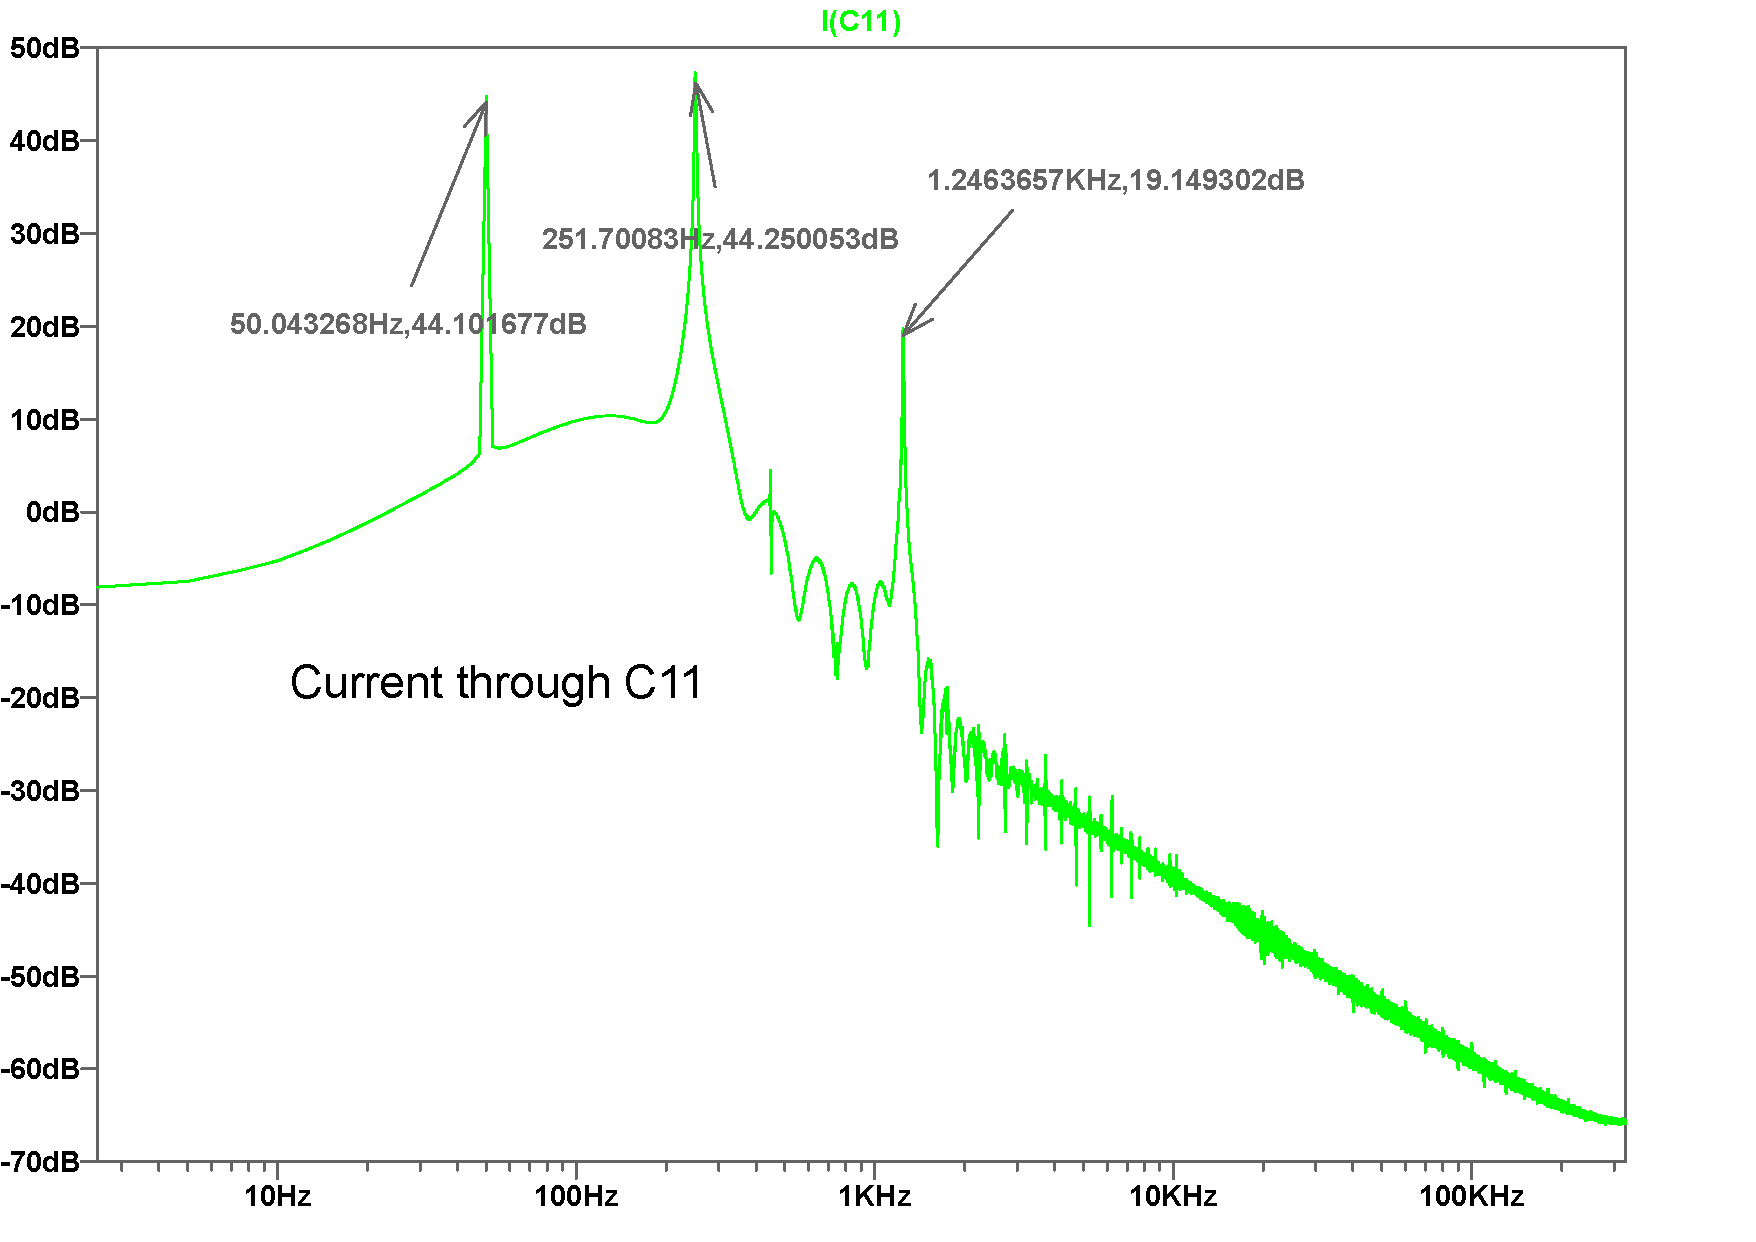
\includegraphics[width=0.70\textwidth]{figures/05_Petersen_earth_faults/Petersen_with_fault_FFT.pdf}
	\caption{FFT of current through capacitor C11}
	\label{fig:Figure13}
\end{figure}

\begin{chaptersummary}
In a resonantly earthed cable network, the Petersen coil compensates the
zero-sequence capacitive earth-fault current. Network asymmetry creates a small
neutral displacement voltage even without a fault. During a solid earth fault (currents like at a shorted circuit at startup),
the healthy phases rise toward line-to-line voltage and the capacitive reactive
power approximately doubles for the first instant. The complete tuning must include transformer and
source impedance, not only the cable capacitance. Fault inception excites
several natural frequencies determined by different inductive and capacitive
paths. For networks without an accessible neutral, a neutral-forming
transformer permits connection of the Petersen coil.
High transient currents arise during the redistribution of charge in the phase-to-earth capacitances. The capacitance of the faulted phase is discharged, while the voltages across the capacitances of the two healthy phases increase to approximately √3 times their normal values. At the higher frequencies excited by the fault, capacitive reactance decreases and inductive reactance increases. These changes contribute to the high initial currents and voltage distortion. The resonant frequencies depend on the inductances and capacitances of the relevant circuit paths.
During the earth fault, the total capacitive reactive power of the healthy phases is approximately twice the prefault three-phase value. As the transient decays, the Petersen coil compensates the additional zero-sequence earth-fault current, while the ordinary charging current remains supplied by the source.
Note: The line inductances in this particular example are modelled without mutual coupling. Including coupling can change the effective fault-path impedance and the initial peak fault current. Compare the coupled and uncoupled models discussed in Section 5.6.
\end{chaptersummary}
